\section*{Přílohy}
\addcontentsline{toc}{section}{Přílohy}
\sectionPriloha{Odvození limitního restitučního faktoru pro podzvukové rychlosti} \label{priloha:odvozeni-limitniho-f}
    Uvažujme vztah pro chybu odhadu stagnační teploty $\varepsilon _{T0}$:
    \begin{equation*}
        \varepsilon _{T0} = 1 - \frac{T + f \frac{u^2}{2 c_p}}{T + \frac{u^2}{2 c_p}}
    \end{equation*}
    \noindent S rostoucí rychlostí proudění dochází i k nárůstu chyby, maxima tedy nabývá při dosažení rychlosti zvuku $a = \sqrt{\kappa r T}$. Označme tuto chybu $\varepsilon _{T0,max}$. Vztah pro její určení lze odvodit dosazením rychlosti zvuku do původní rovnice:
    \begin{align*}
        \varepsilon _{T0,max} &= 1 - \frac{T + f \frac{\kappa r T}{2 \frac{\kappa r}{\kappa - 1}}}{T + \frac{\kappa r T}{2 \frac{\kappa r}{\kappa - 1}}} \\
        \varepsilon _{T0,max} &= 1 - \frac{1 + f \frac{\kappa - 1}{2}}{1 + \frac{\kappa - 1}{2}}
    \end{align*}
    \noindent Maximální chyba je tedy pouze funkcí restitučního faktoru a Poissonovy konstanty. Budeme-li pro konkrétní $\kappa$ požadovat, aby chyba nepřekročila limitní hodnotu $\varepsilon _{T0,lim}$, pak lze s využitím vztahu pro $\varepsilon _{T,max}$ odvodit i limitní restituční faktor $f_{lim}$:
    \begin{align*}
        \varepsilon _{T0,lim} &= 1 - \frac{1 + f_{lim} \frac{\kappa - 1}{2}}{1 + \frac{\kappa - 1}{2}} \\
        \brac{1 - \varepsilon _{T0,lim}} \brac{1 + \frac{\kappa - 1}{2}} &= 1 + f_{lim} \frac{\kappa - 1}{2} \\
        f_{lim} &= \frac{2}{\kappa - 1} \Brac{\brac{1 - \varepsilon _{T0,lim}} \brac{1 + \frac{\kappa - 1}{2}} - 1}
    \end{align*}
    \noindent Bude-li hodnota restitučního faktoru vybraného teplotního čidla $\geq f_{lim}$, potom bude splněna podmínka limitní chyby pro libovolnou podzvukovou rychlost i statickou teplotu.
    \newpage

\sectionPriloha{Sonda bez stínění čidla B} \label{fig:sonda-bez-stineni-B-vykres}
    \begin{figure}[ht!]
        \centering
        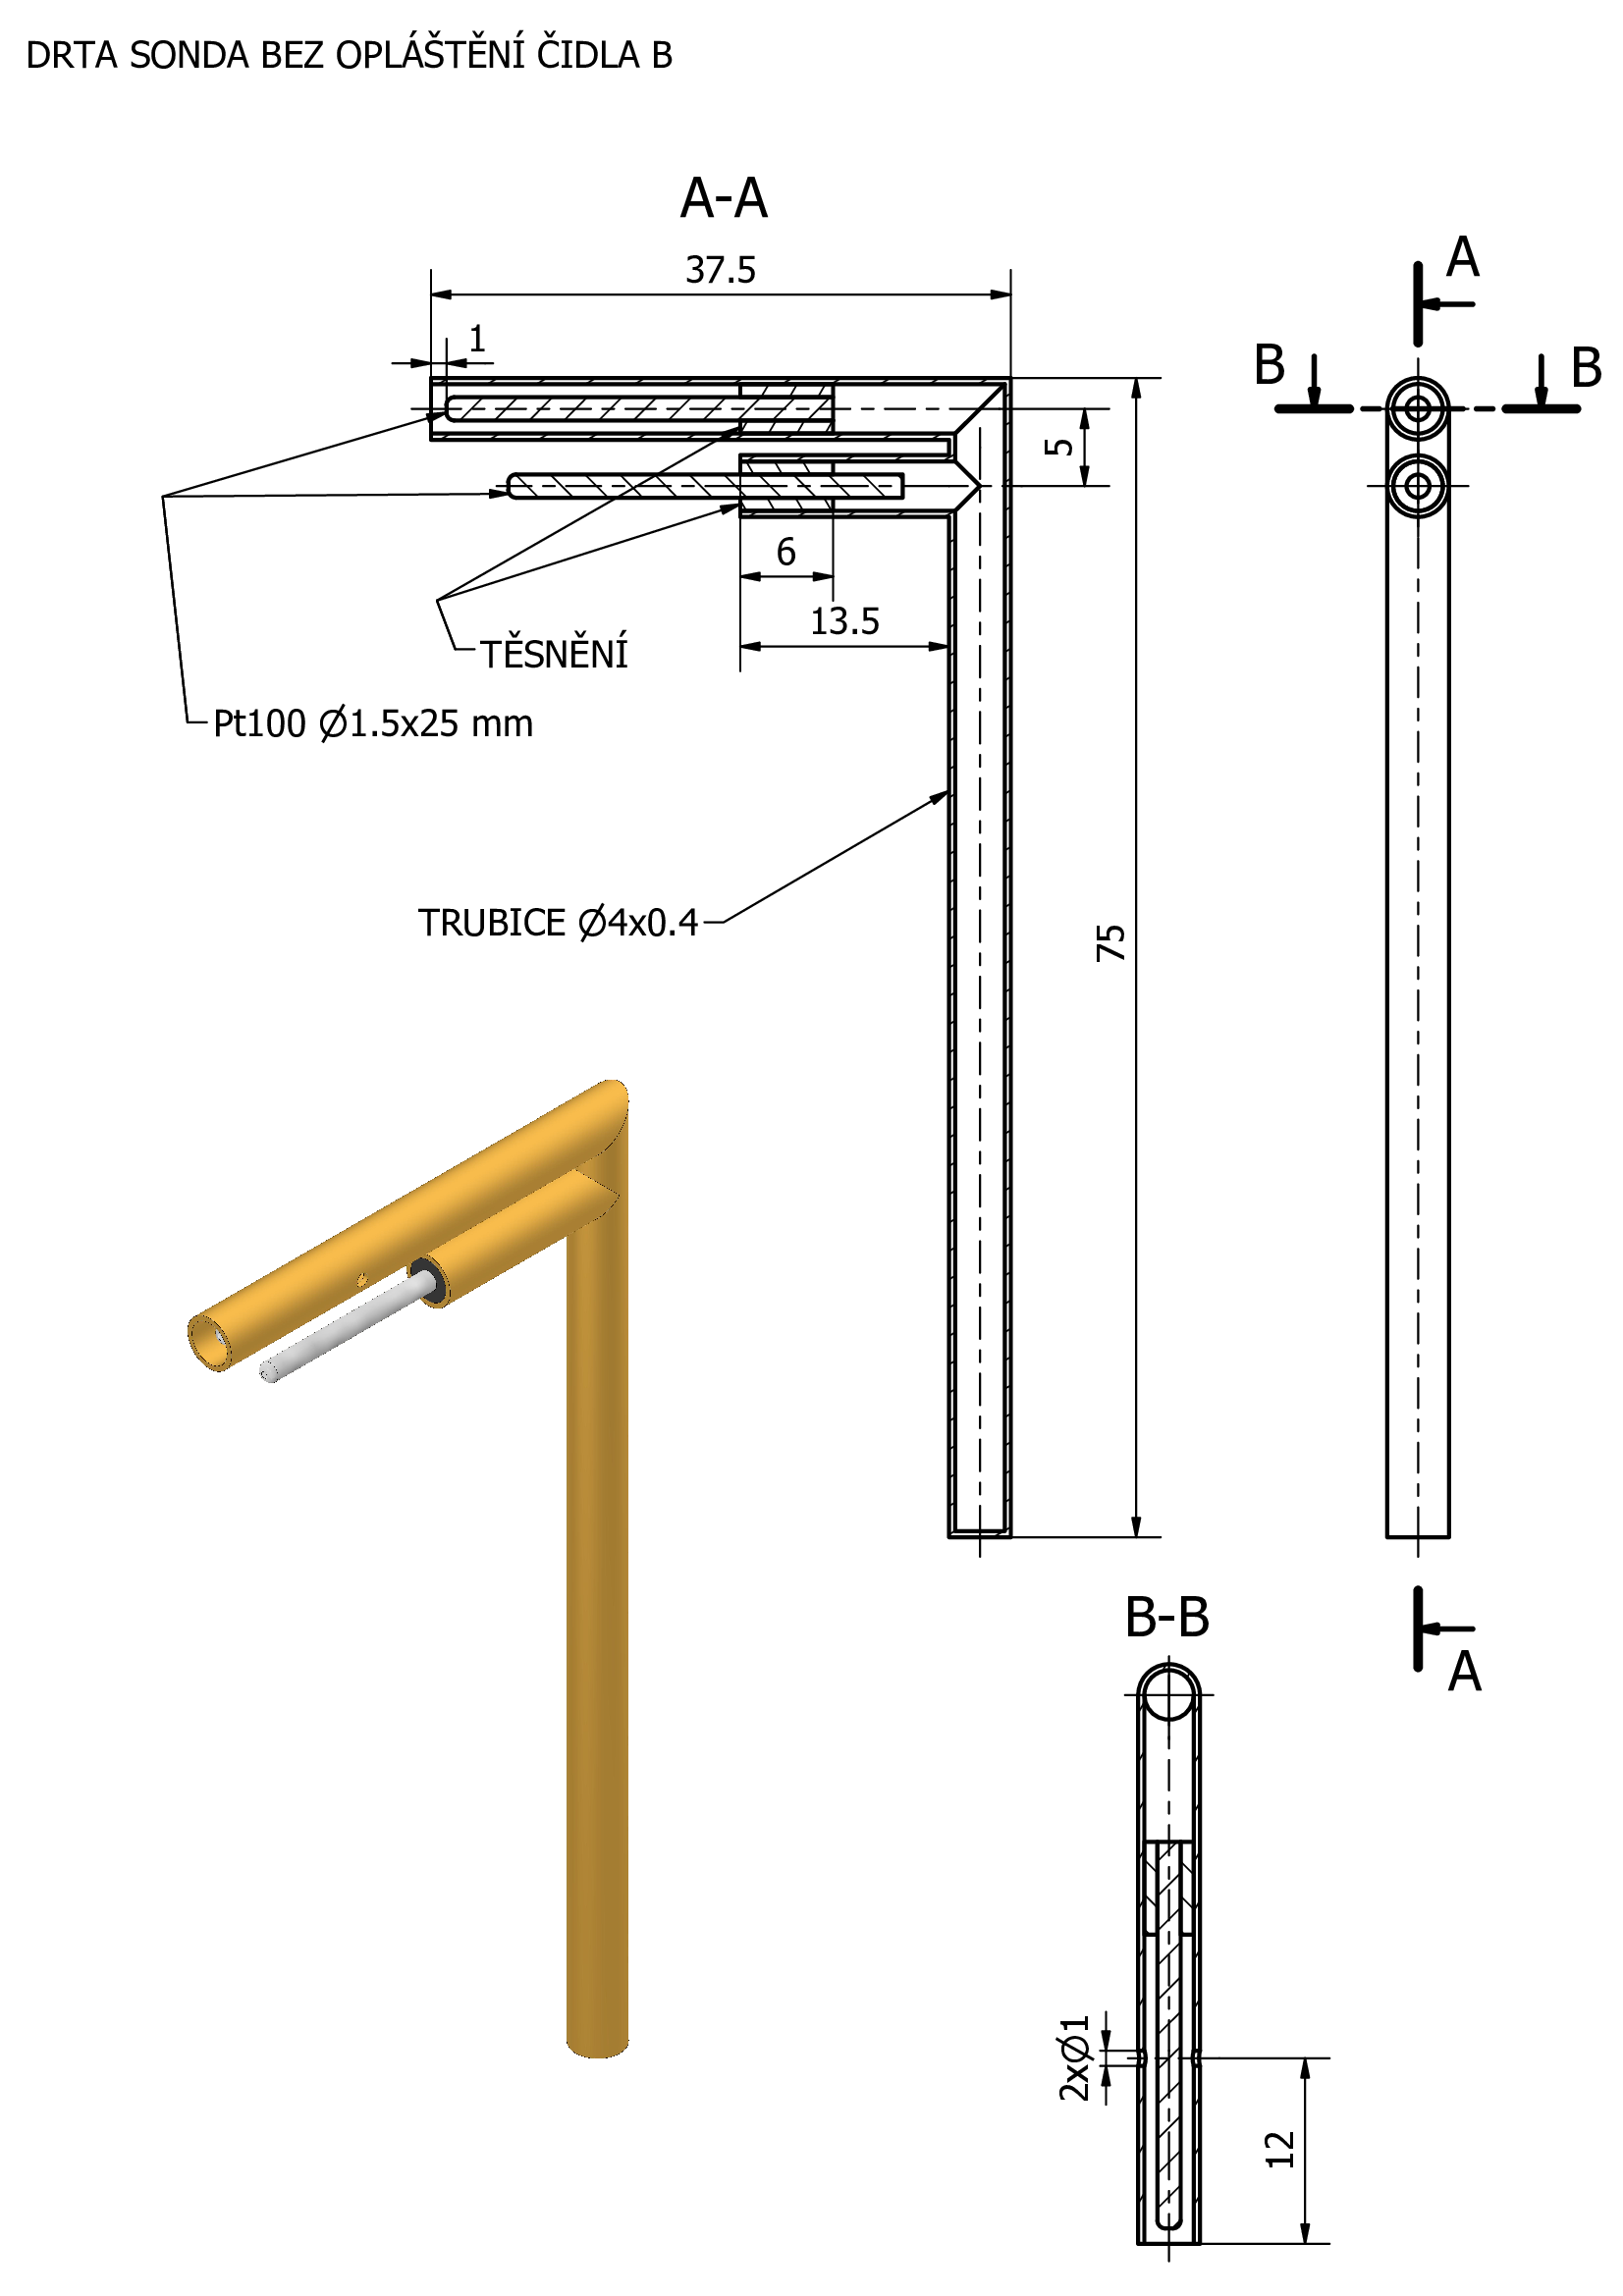
\includegraphics[width=\textwidth]{400_SIMULACE_KONSTRUKCNICH_UPRAV/Vykresy_rendery/Sonda_bez_stineni_B_vykres.png}
        
    \end{figure}
    \newpage
\sectionPriloha{Sonda se stíněním čidla B} \label{fig:sonda-se-stinenim-B-vykres}
    \begin{figure}[ht!]
        \centering
        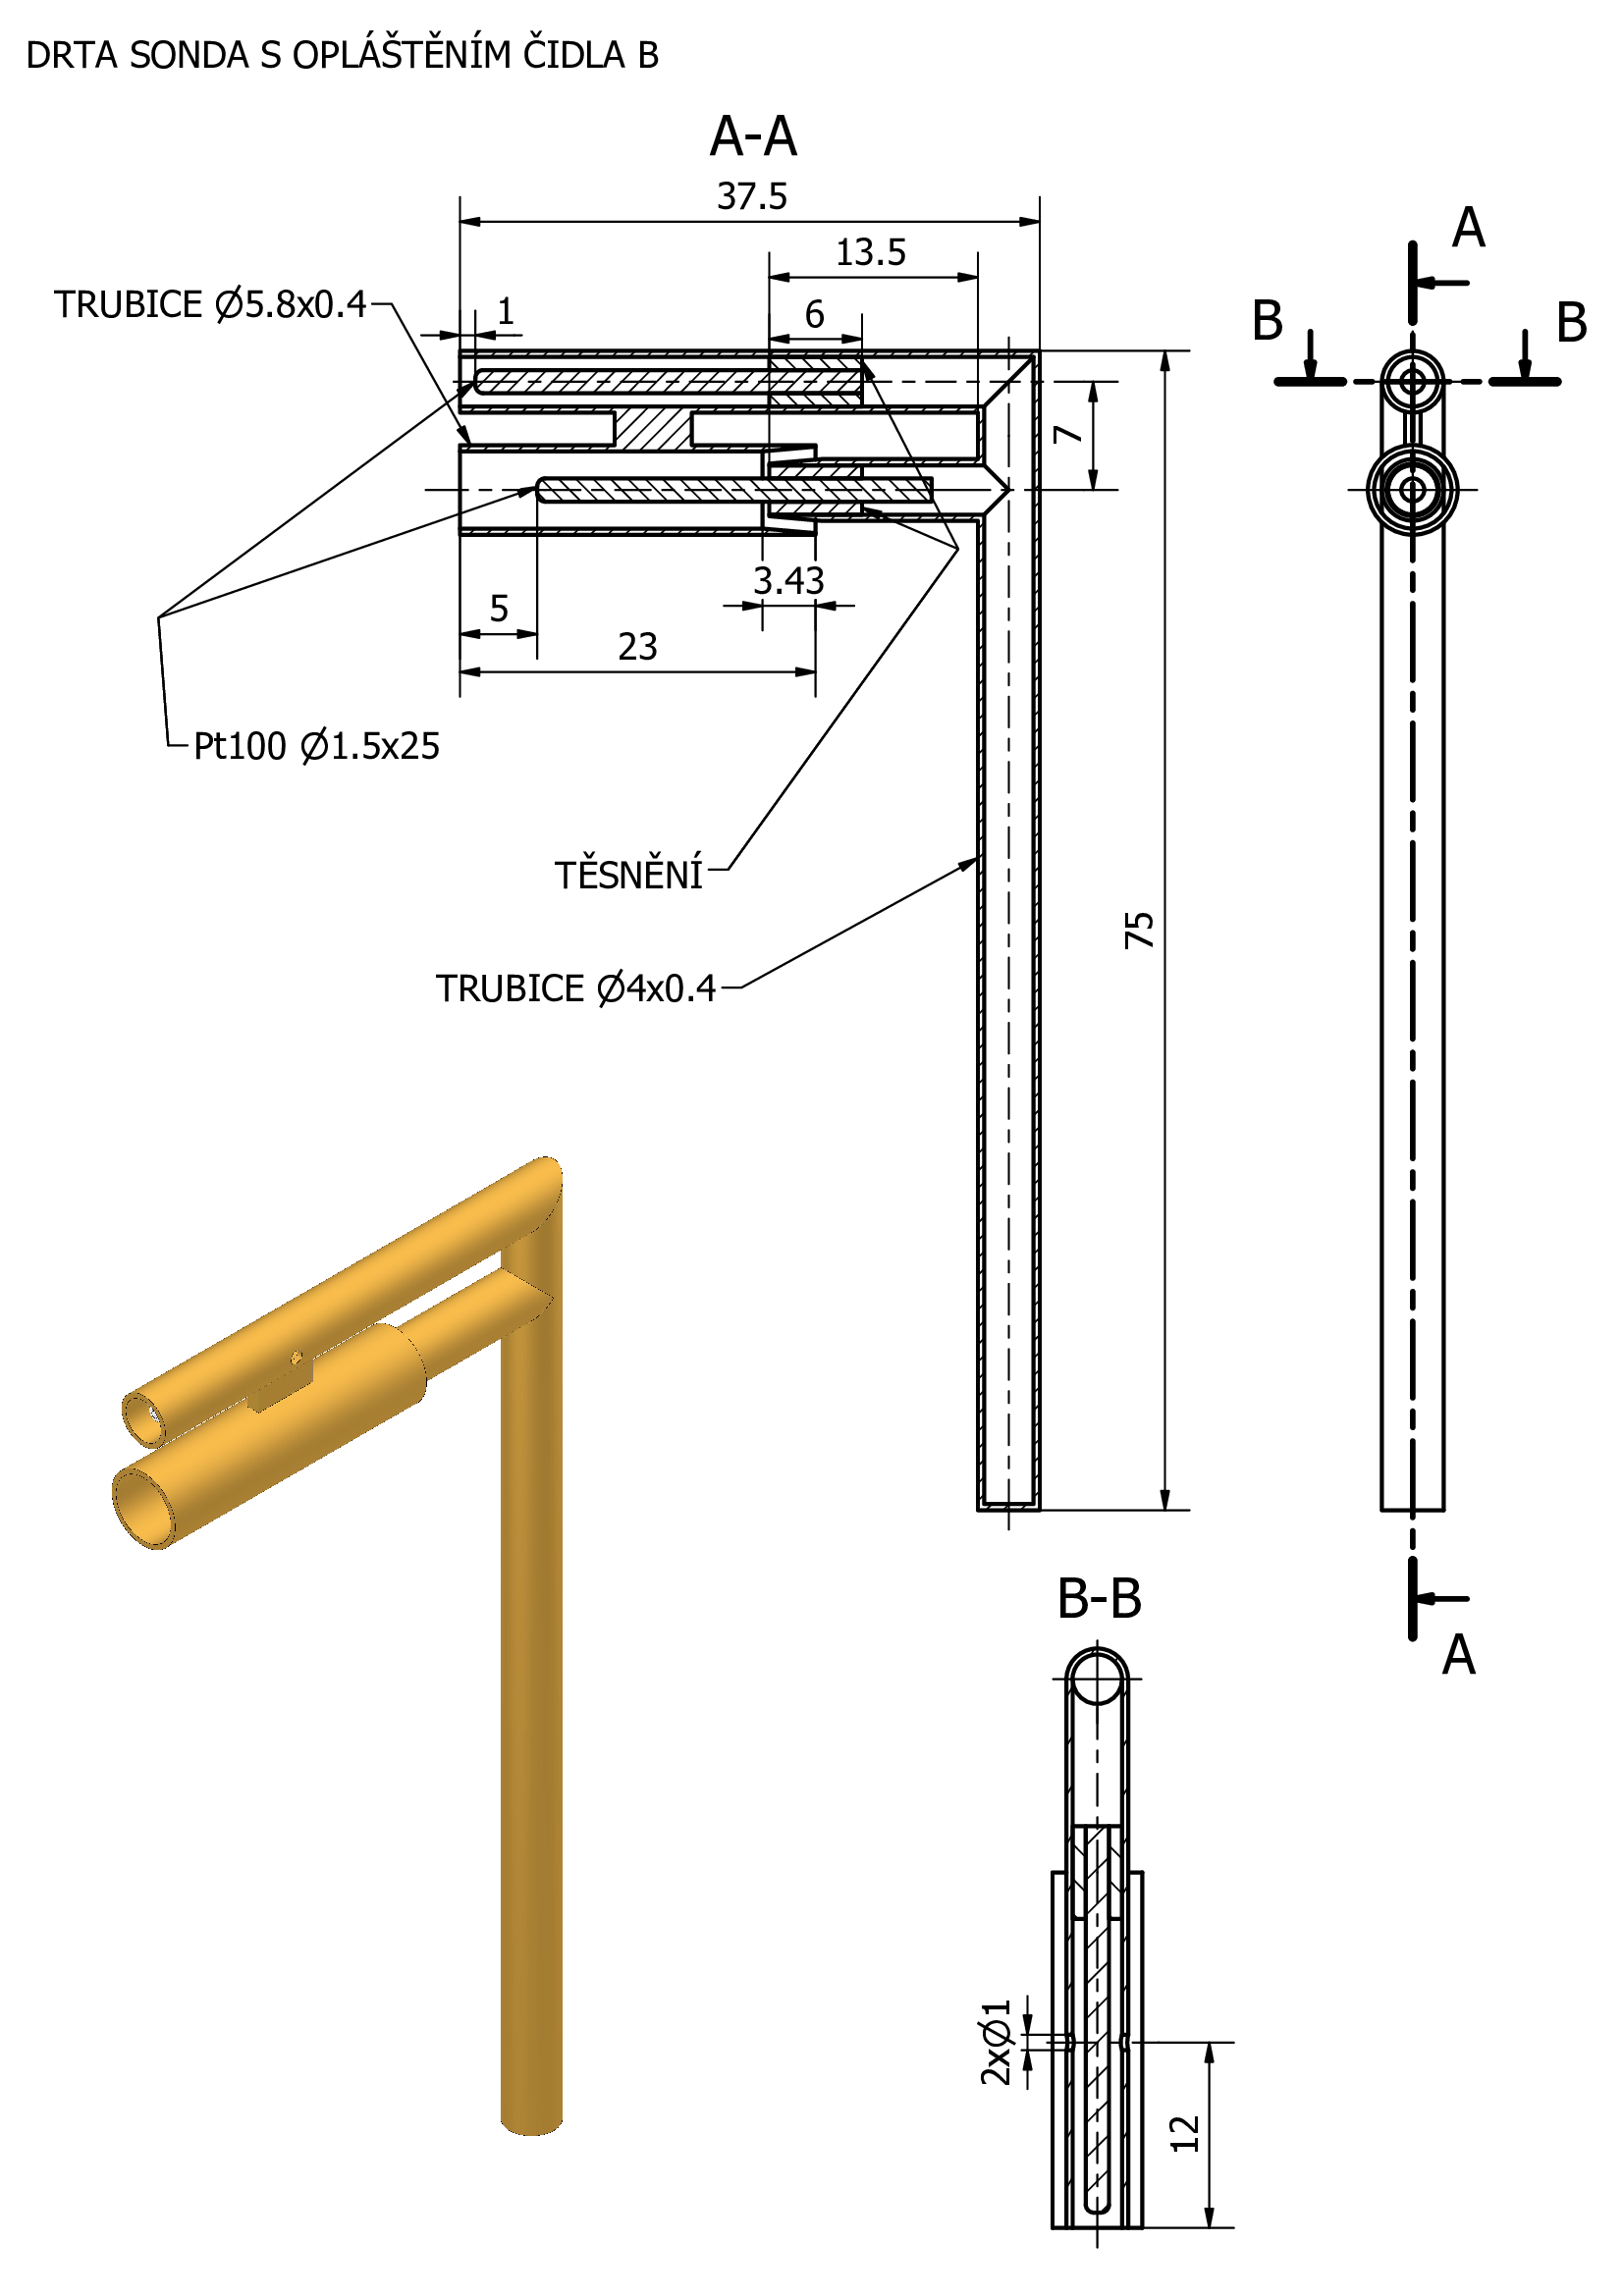
\includegraphics[width=\textwidth]{400_SIMULACE_KONSTRUKCNICH_UPRAV/Vykresy_rendery/Sonda_se_stinenim_B_vykres.png}
        
    \end{figure}
    \newpage
\sectionPriloha{Sonda s rozšířeným stíněním čidla B} \label{fig:sonda-s-rozsirenym-stinenim-B-vykres}
    \begin{figure}[ht!]
        \centering
        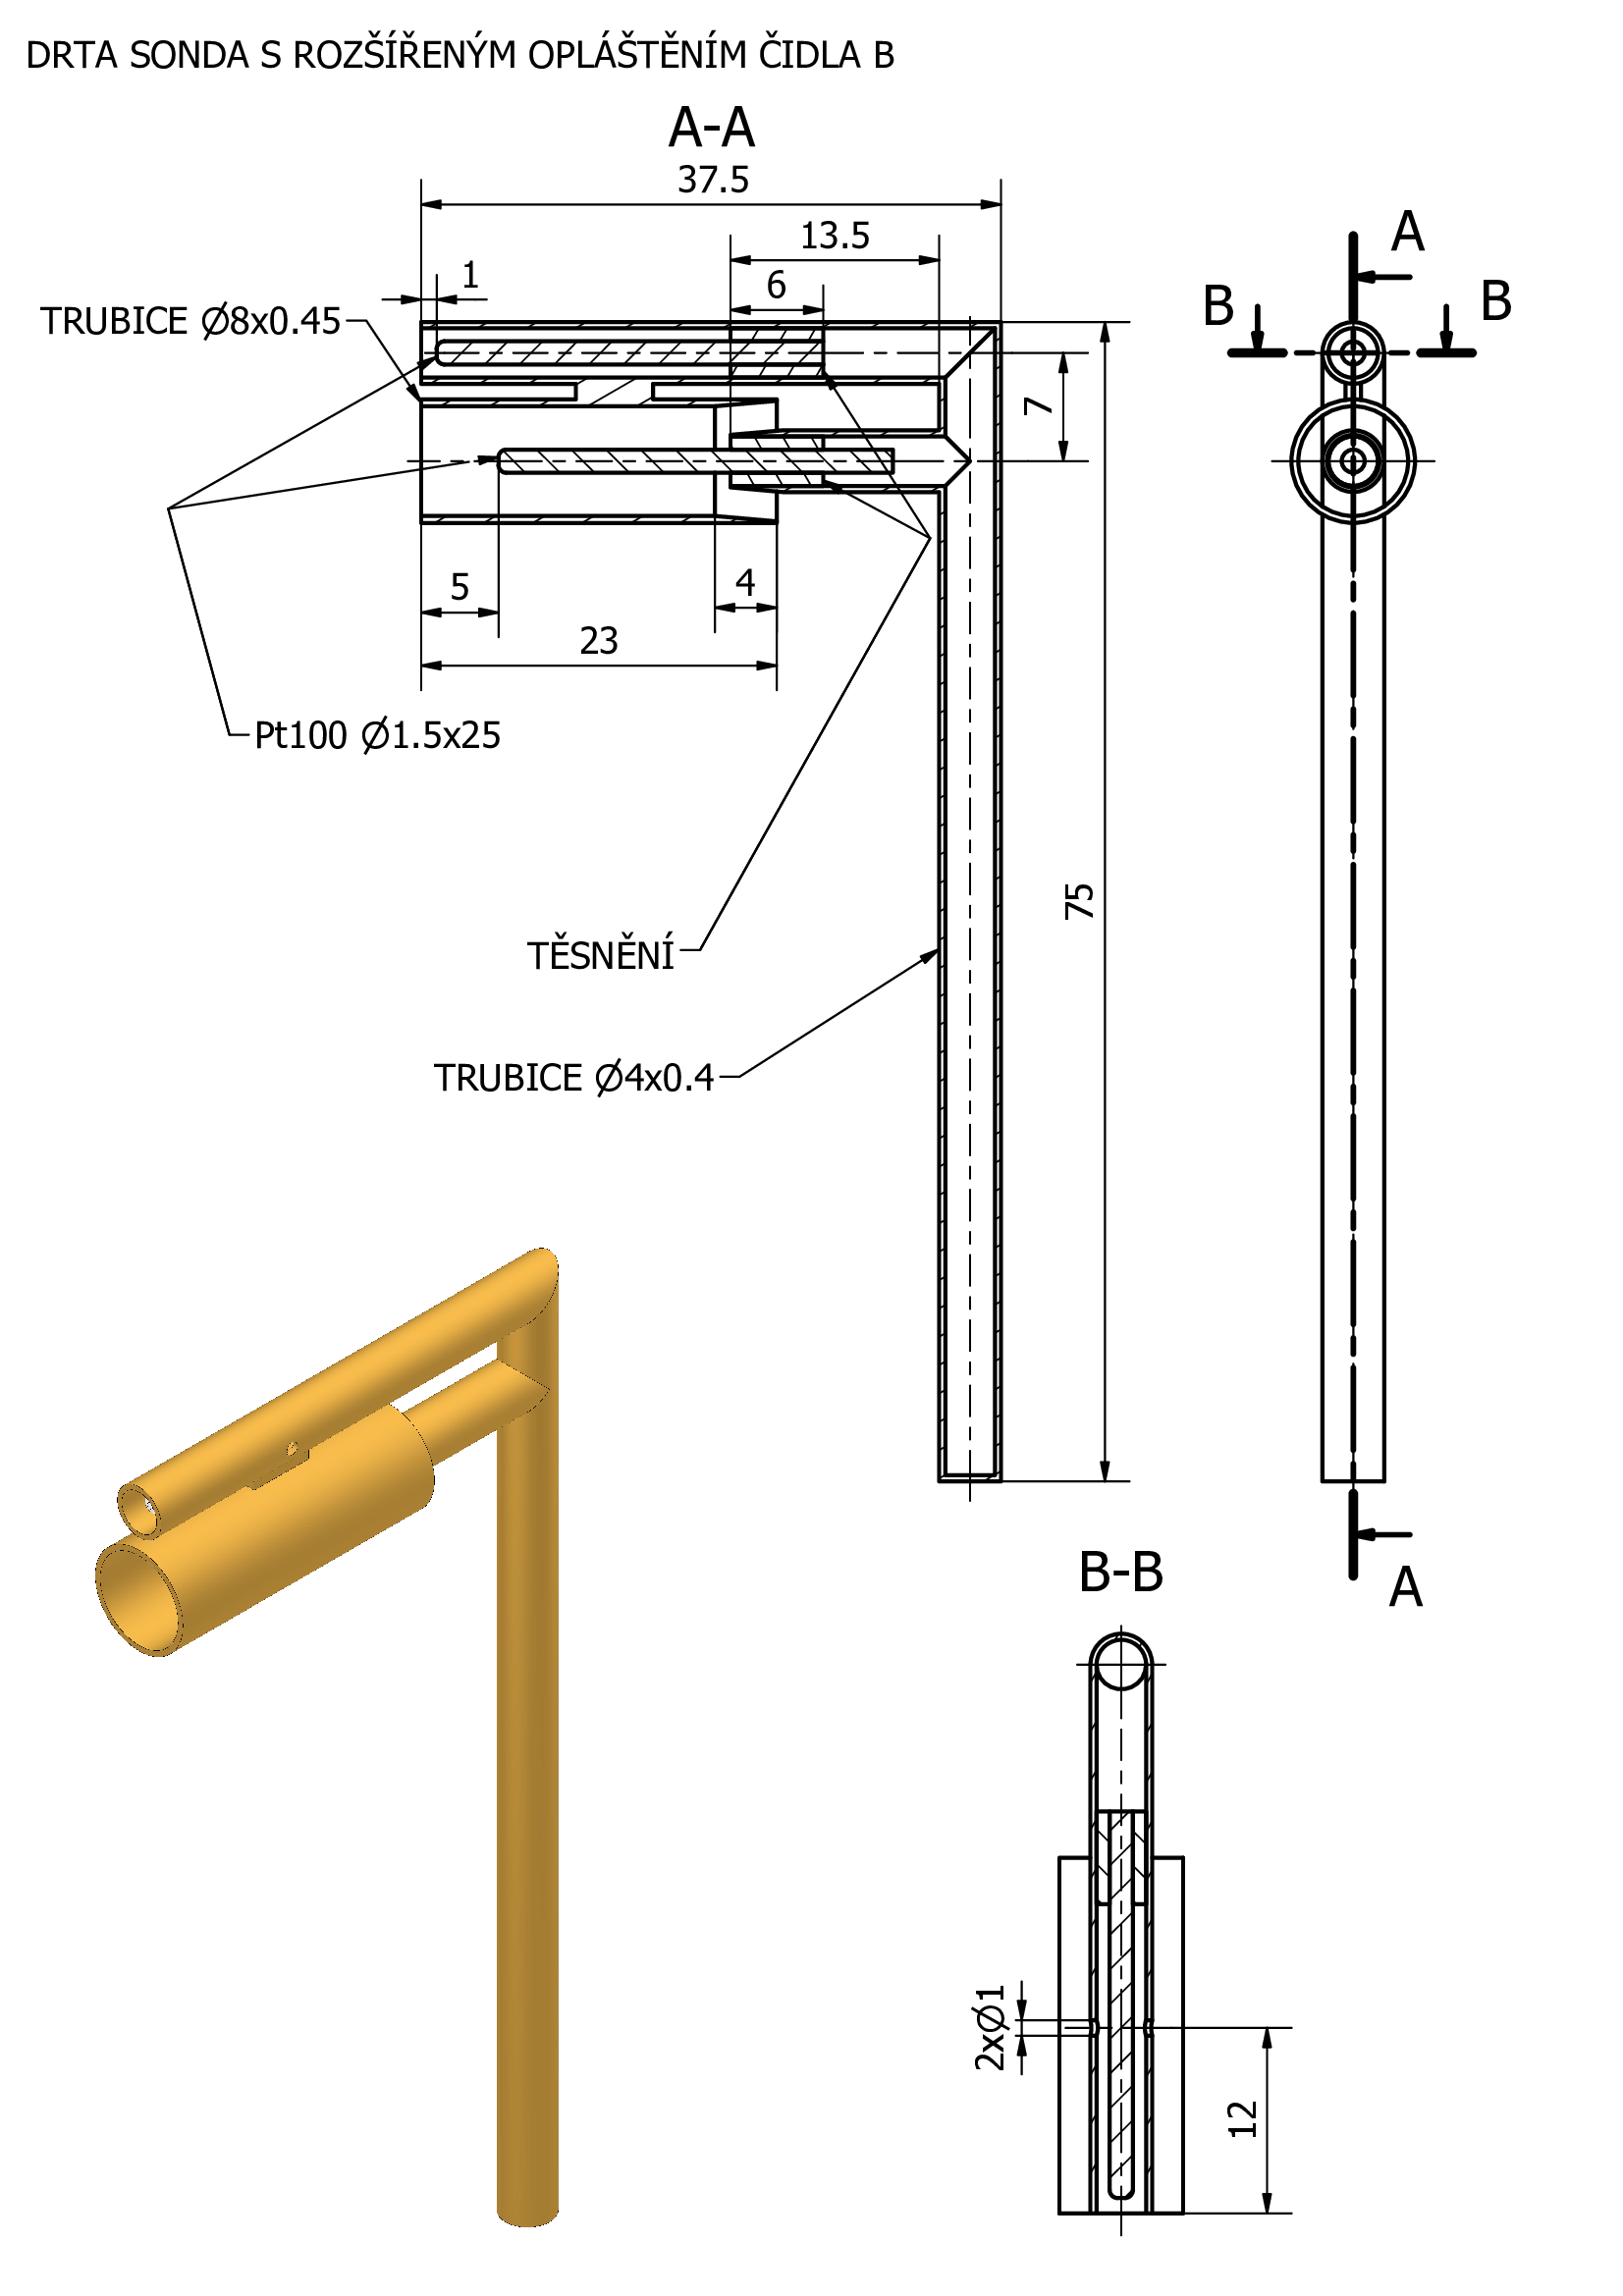
\includegraphics[width=\textwidth]{400_SIMULACE_KONSTRUKCNICH_UPRAV/Vykresy_rendery/Sonda_s_rozsirenym_stinenim_B_vykres.png}
        
    \end{figure}
    \newpage
\sectionPriloha{Stínění čidla B} \label{fig:prumer-stineni-B-vykres}
    \begin{figure}[ht!]
        \centering
        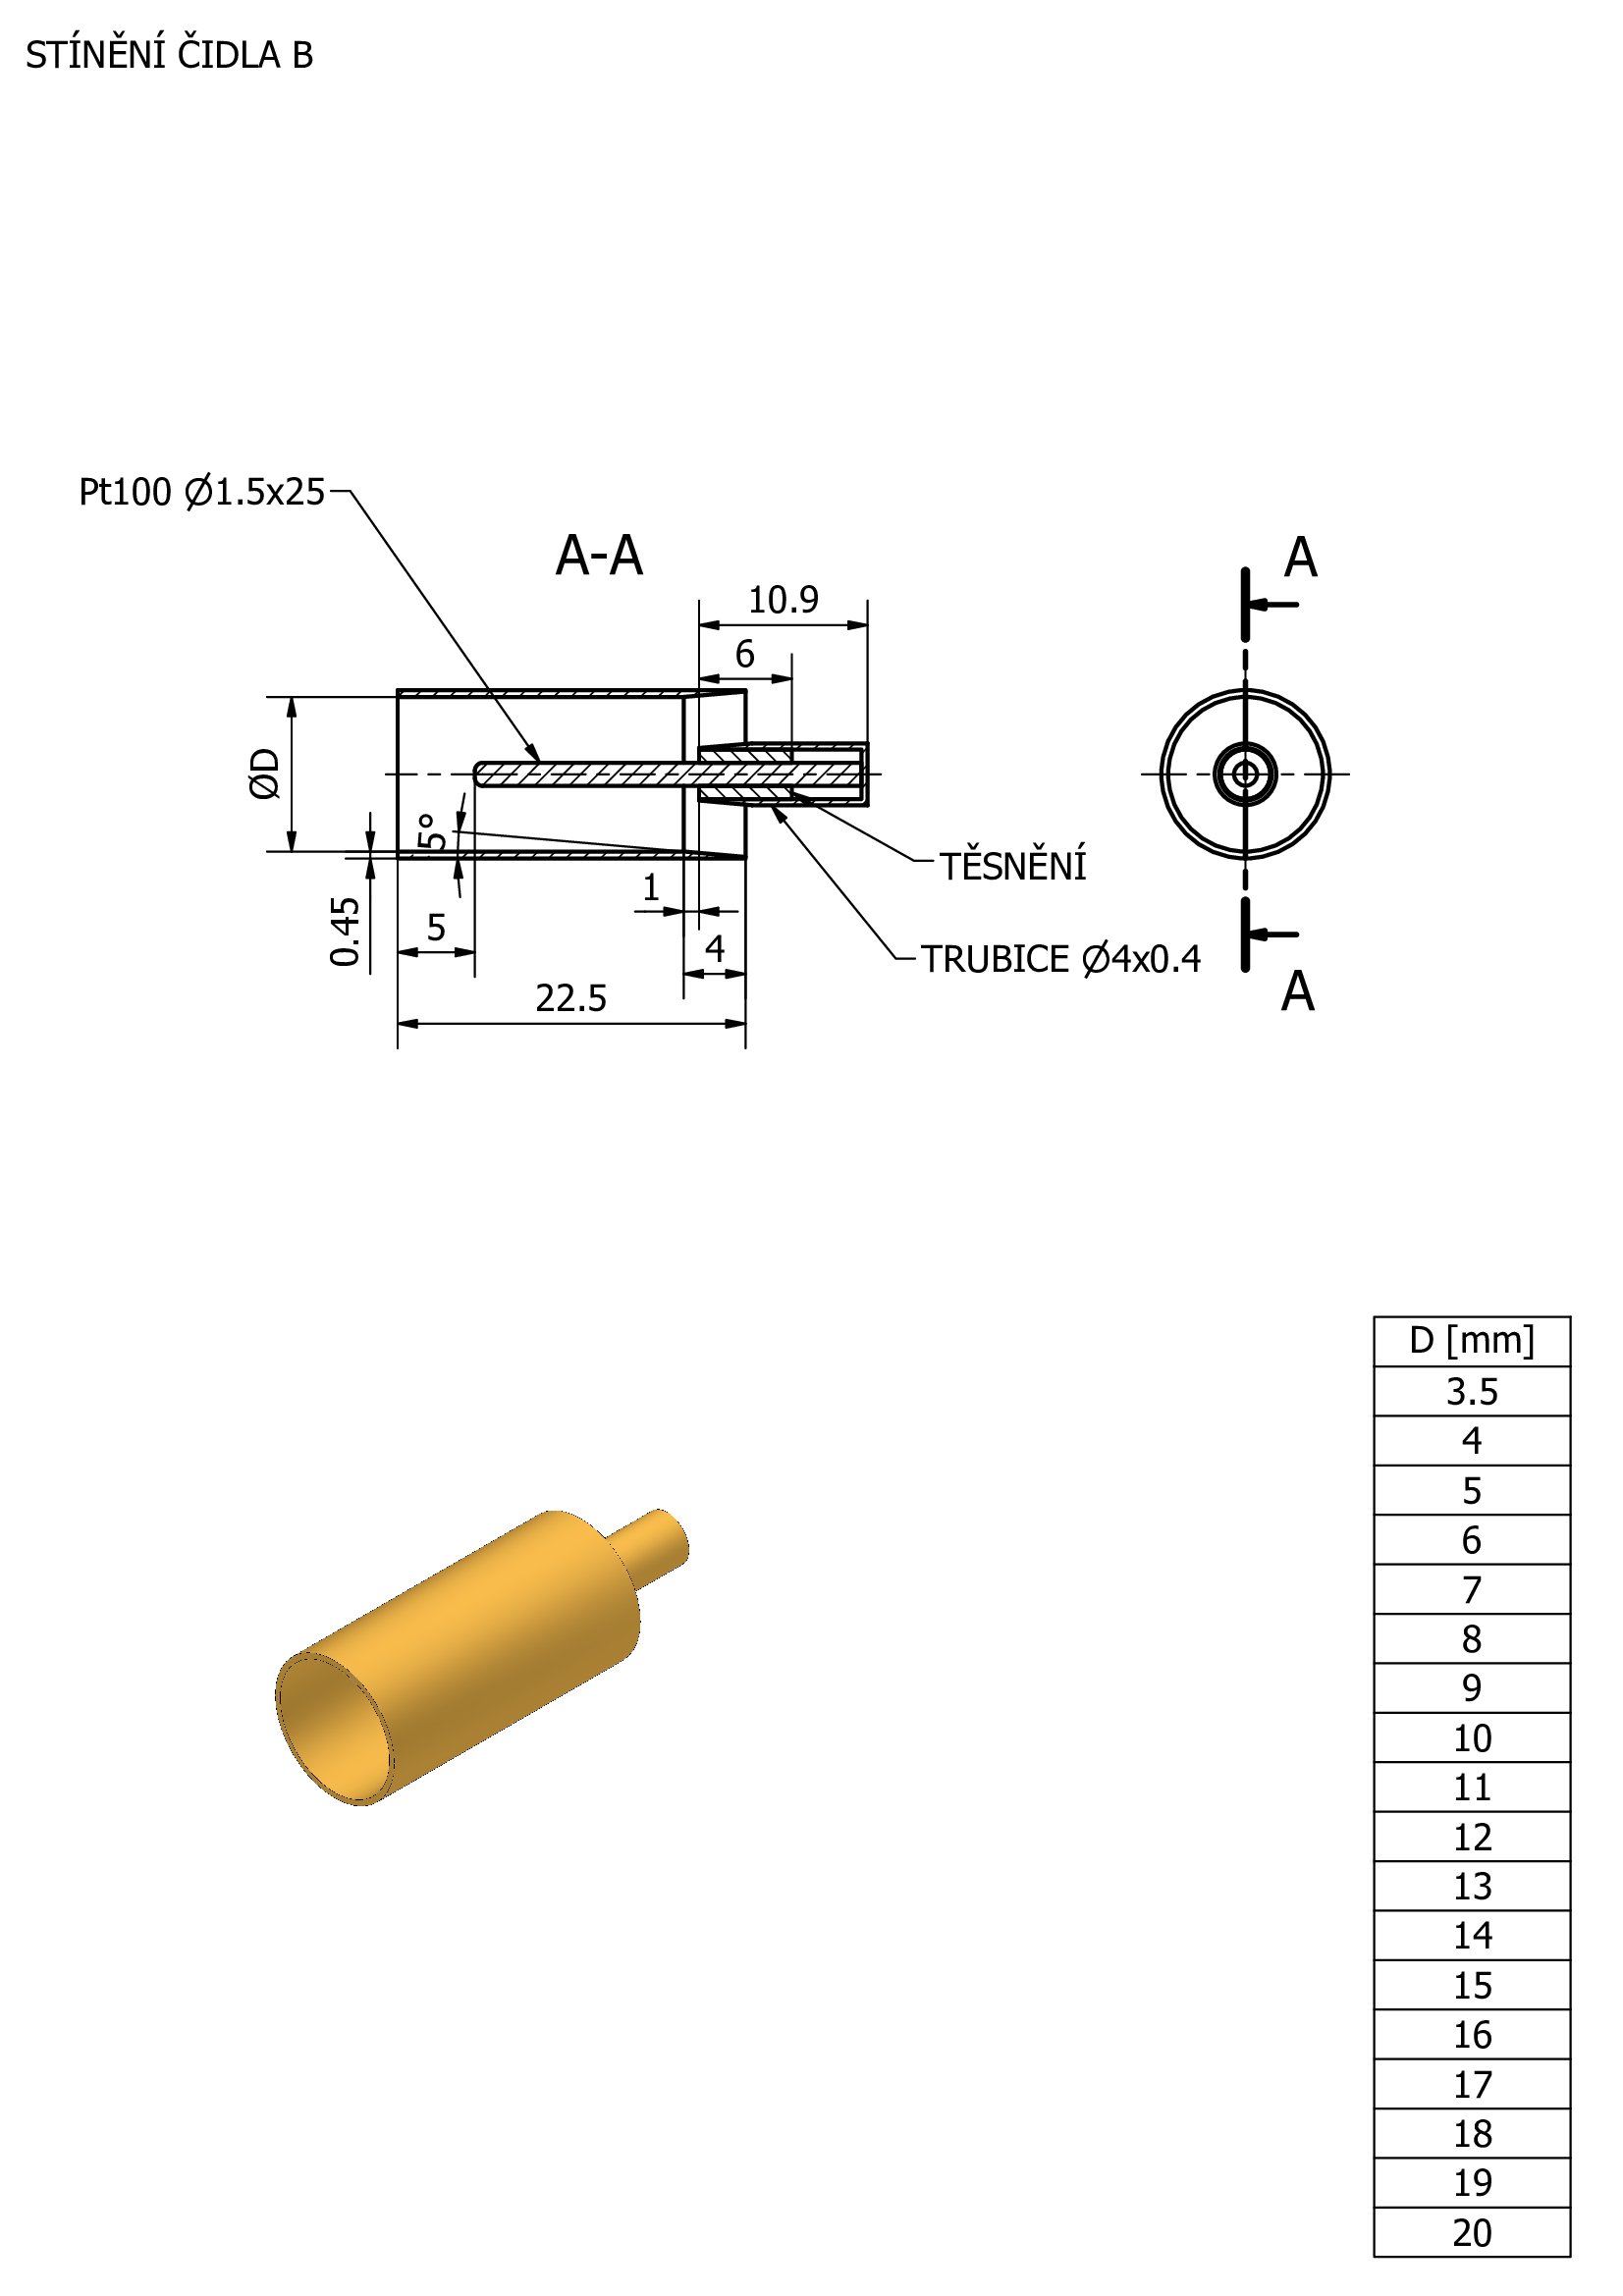
\includegraphics[width=\textwidth]{400_SIMULACE_KONSTRUKCNICH_UPRAV/Vykresy_rendery/Prumer_stineni_B_vykres.png}
        
    \end{figure}
    \newpage
\sectionPriloha{Stínění čidla A} \label{fig:prumer-stineni-A-vykres}
    \begin{figure}[ht!]
        \centering
        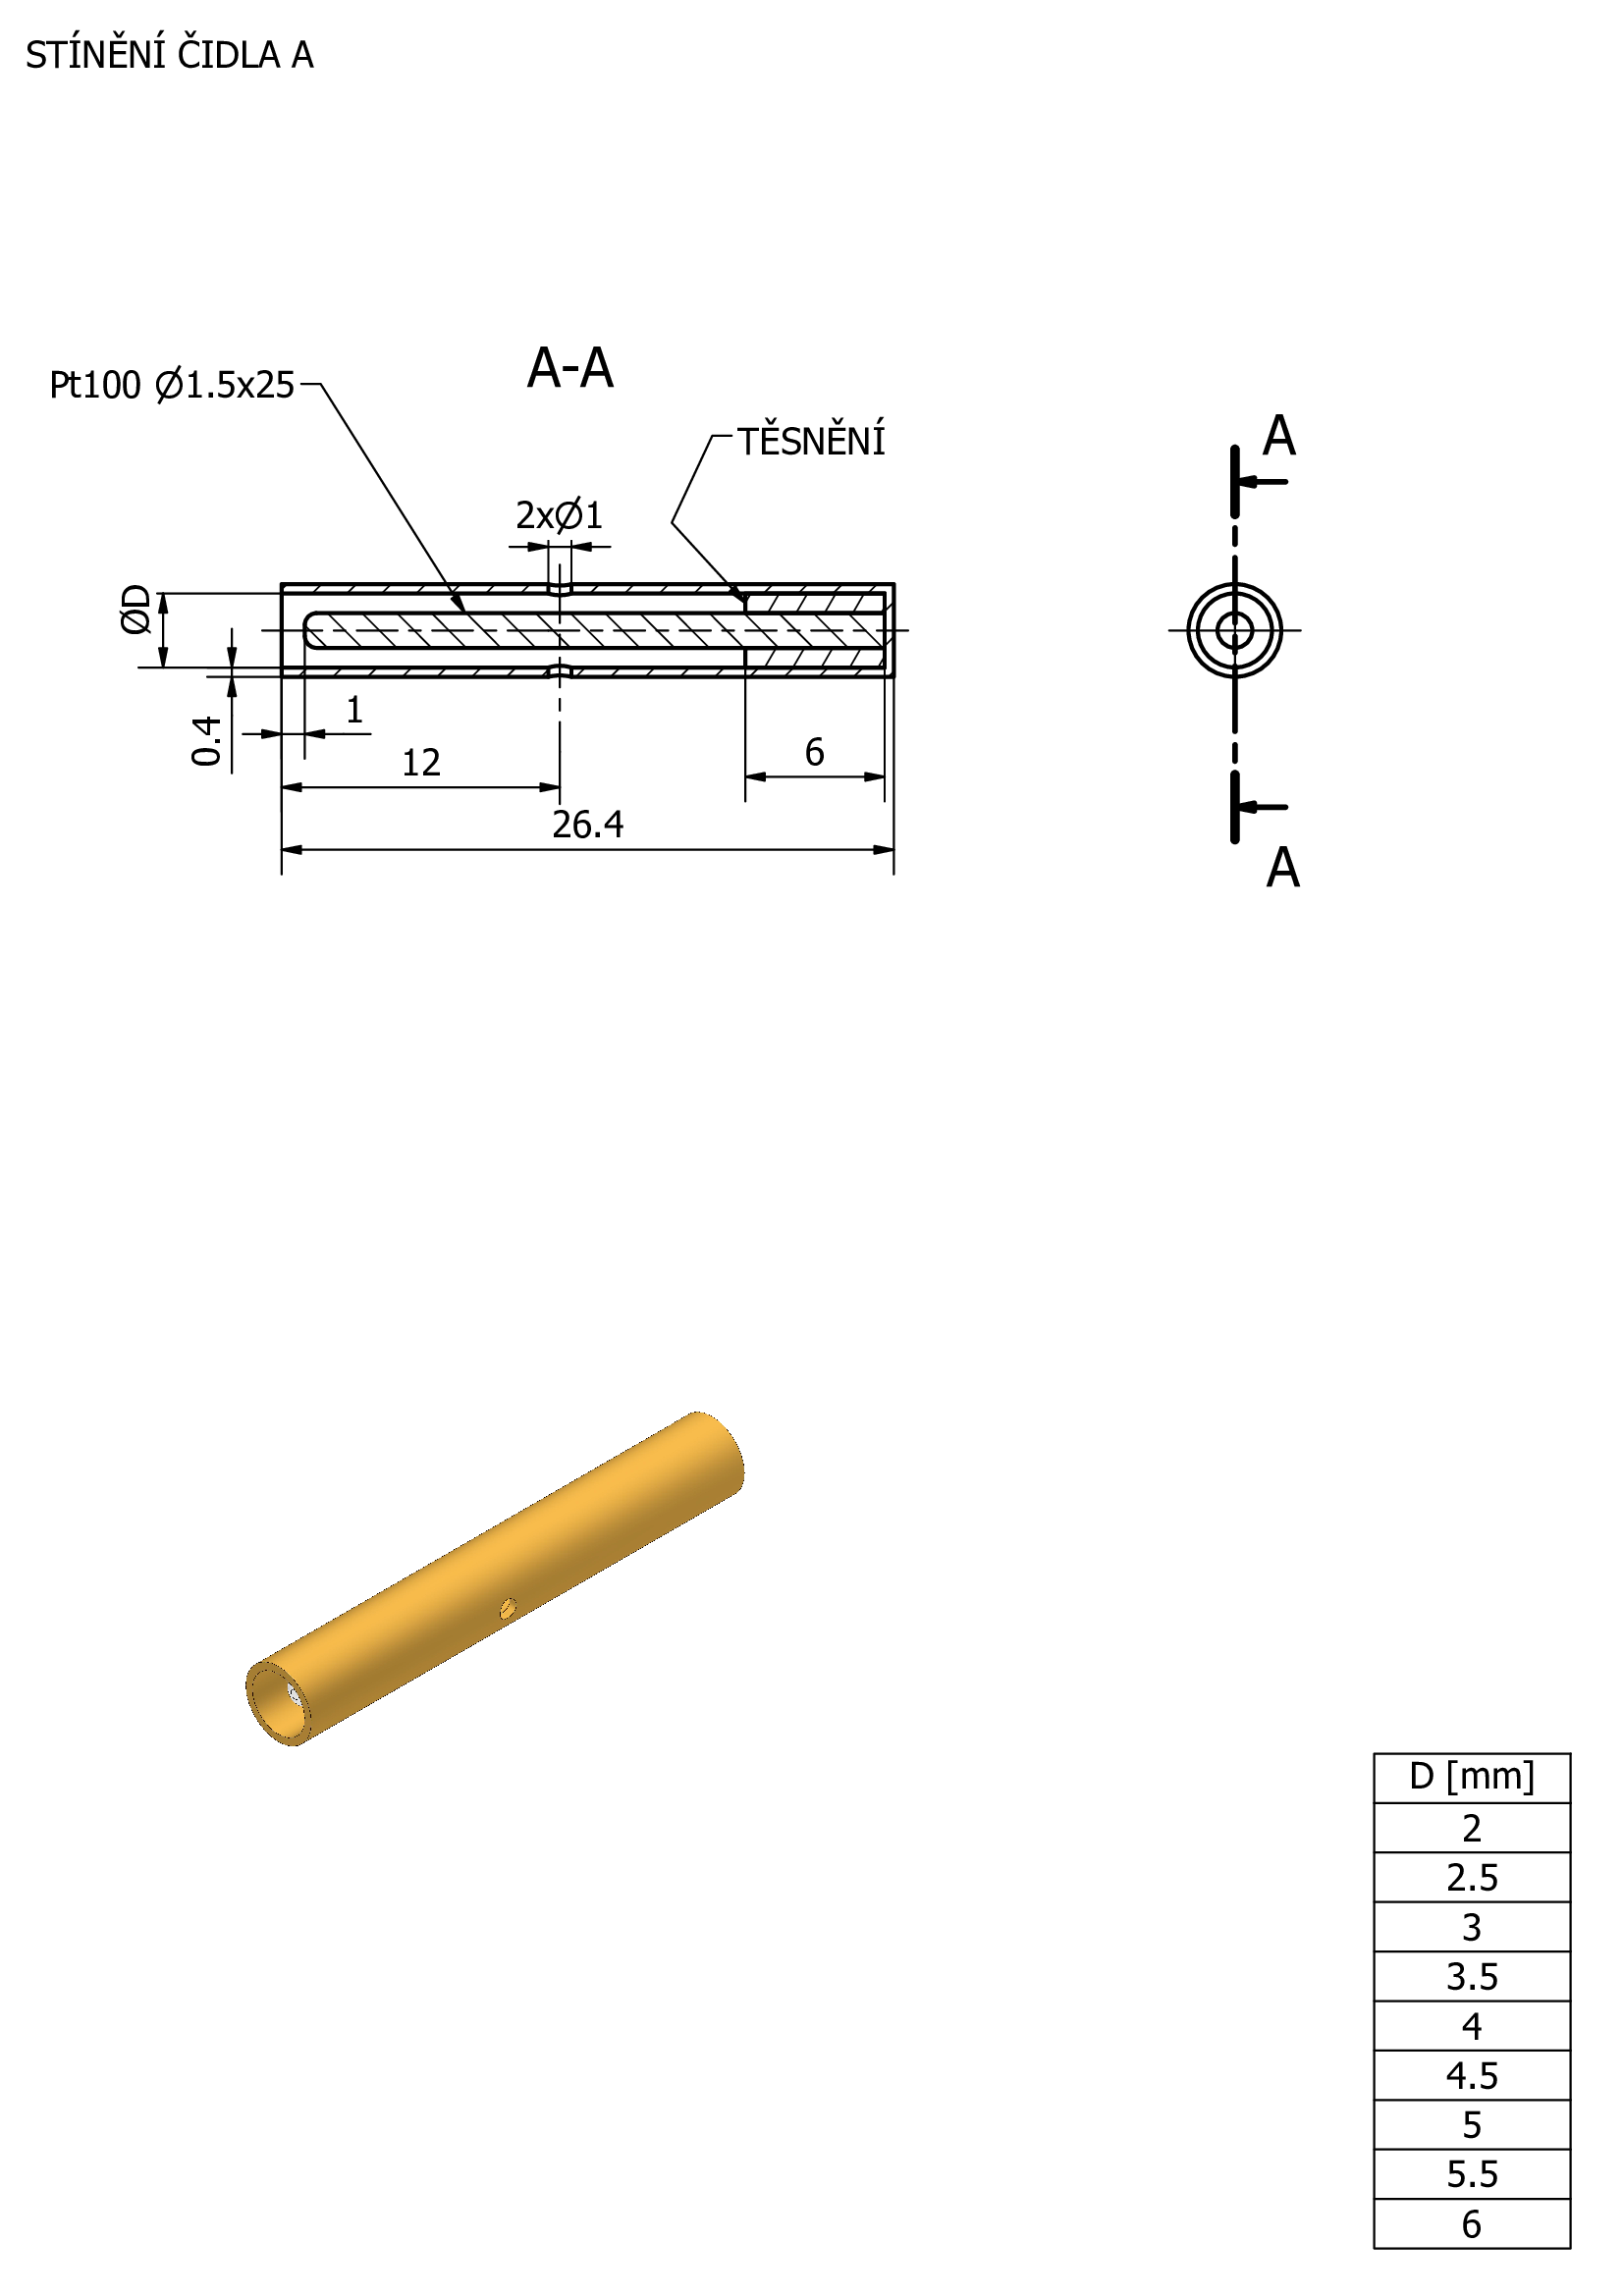
\includegraphics[width=\textwidth]{400_SIMULACE_KONSTRUKCNICH_UPRAV/Vykresy_rendery/Prumer_stineni_A_vykres.png}
        
    \end{figure}
    \newpage
\sectionPriloha{Odvětrání čidla A} \label{fig:odvetrani-A-vykres}
    \begin{figure}[ht!]
        \centering
        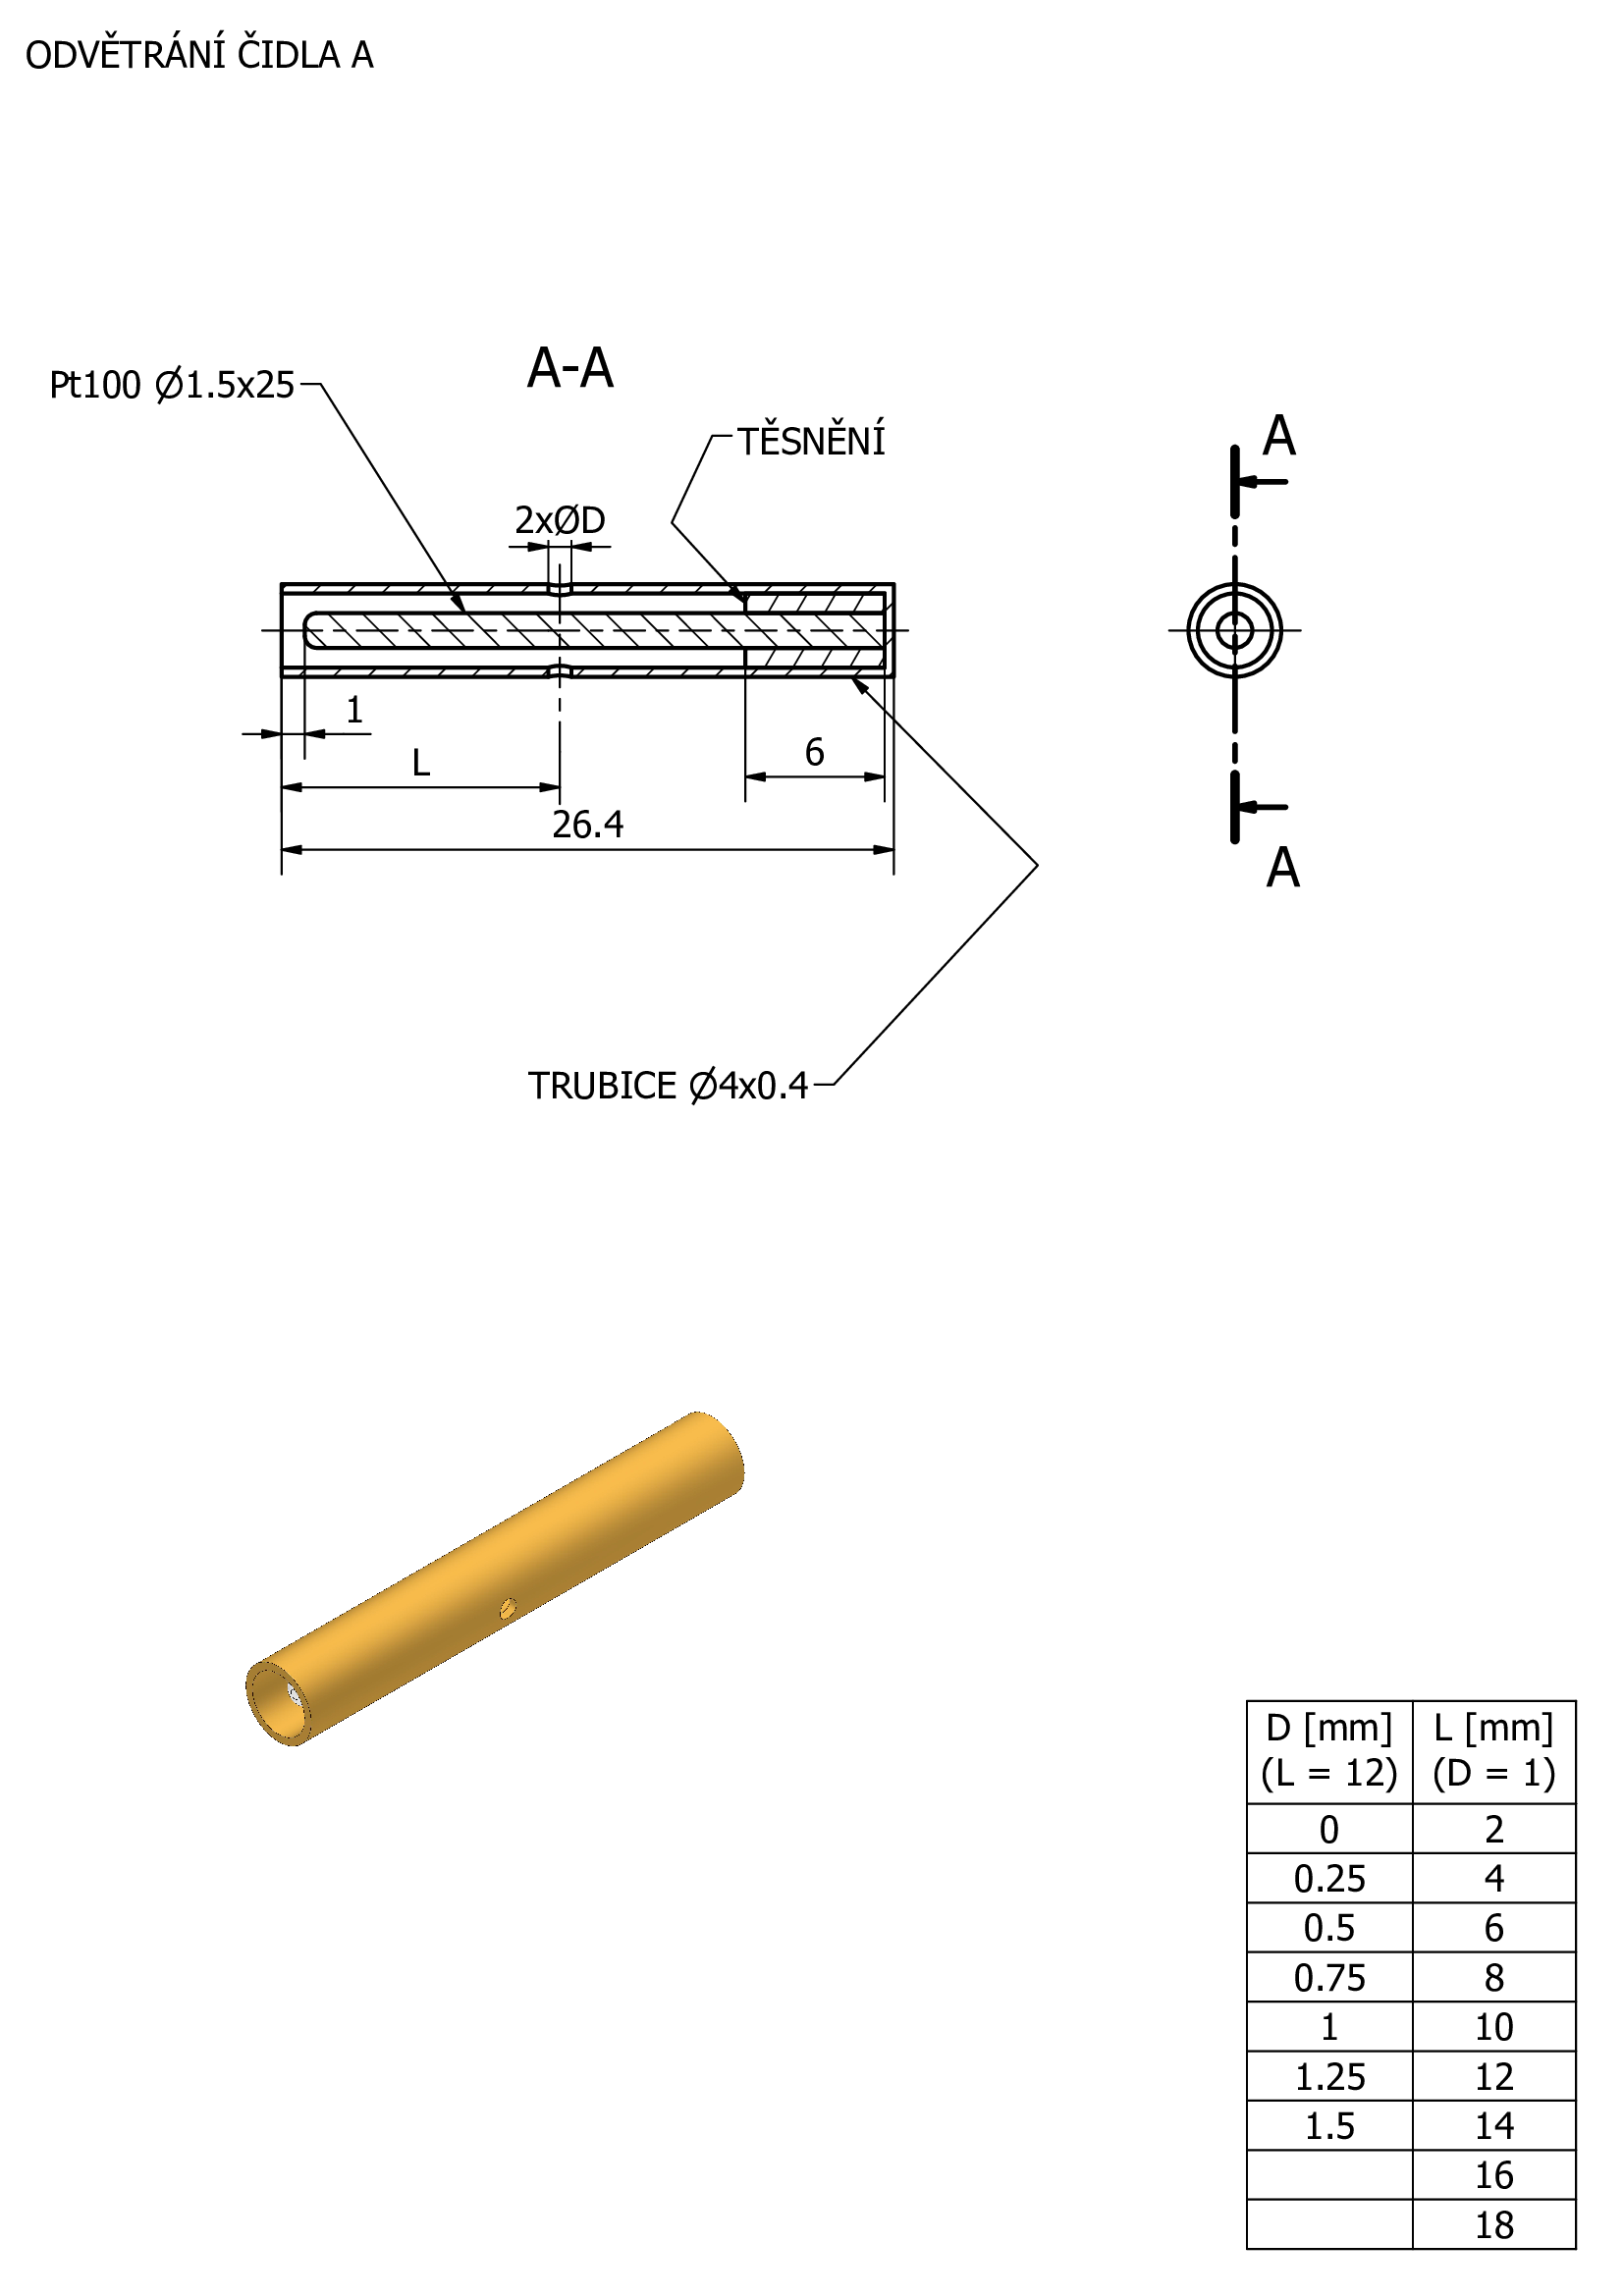
\includegraphics[width=\textwidth]{400_SIMULACE_KONSTRUKCNICH_UPRAV/Vykresy_rendery/Odvetrani_A_vykres.png}
        
    \end{figure}
    \newpage
\sectionPriloha{Divergentní vstup čidla A} \label{fig:difuzor-A-vykres}
    \begin{figure}[ht!]
        \centering
        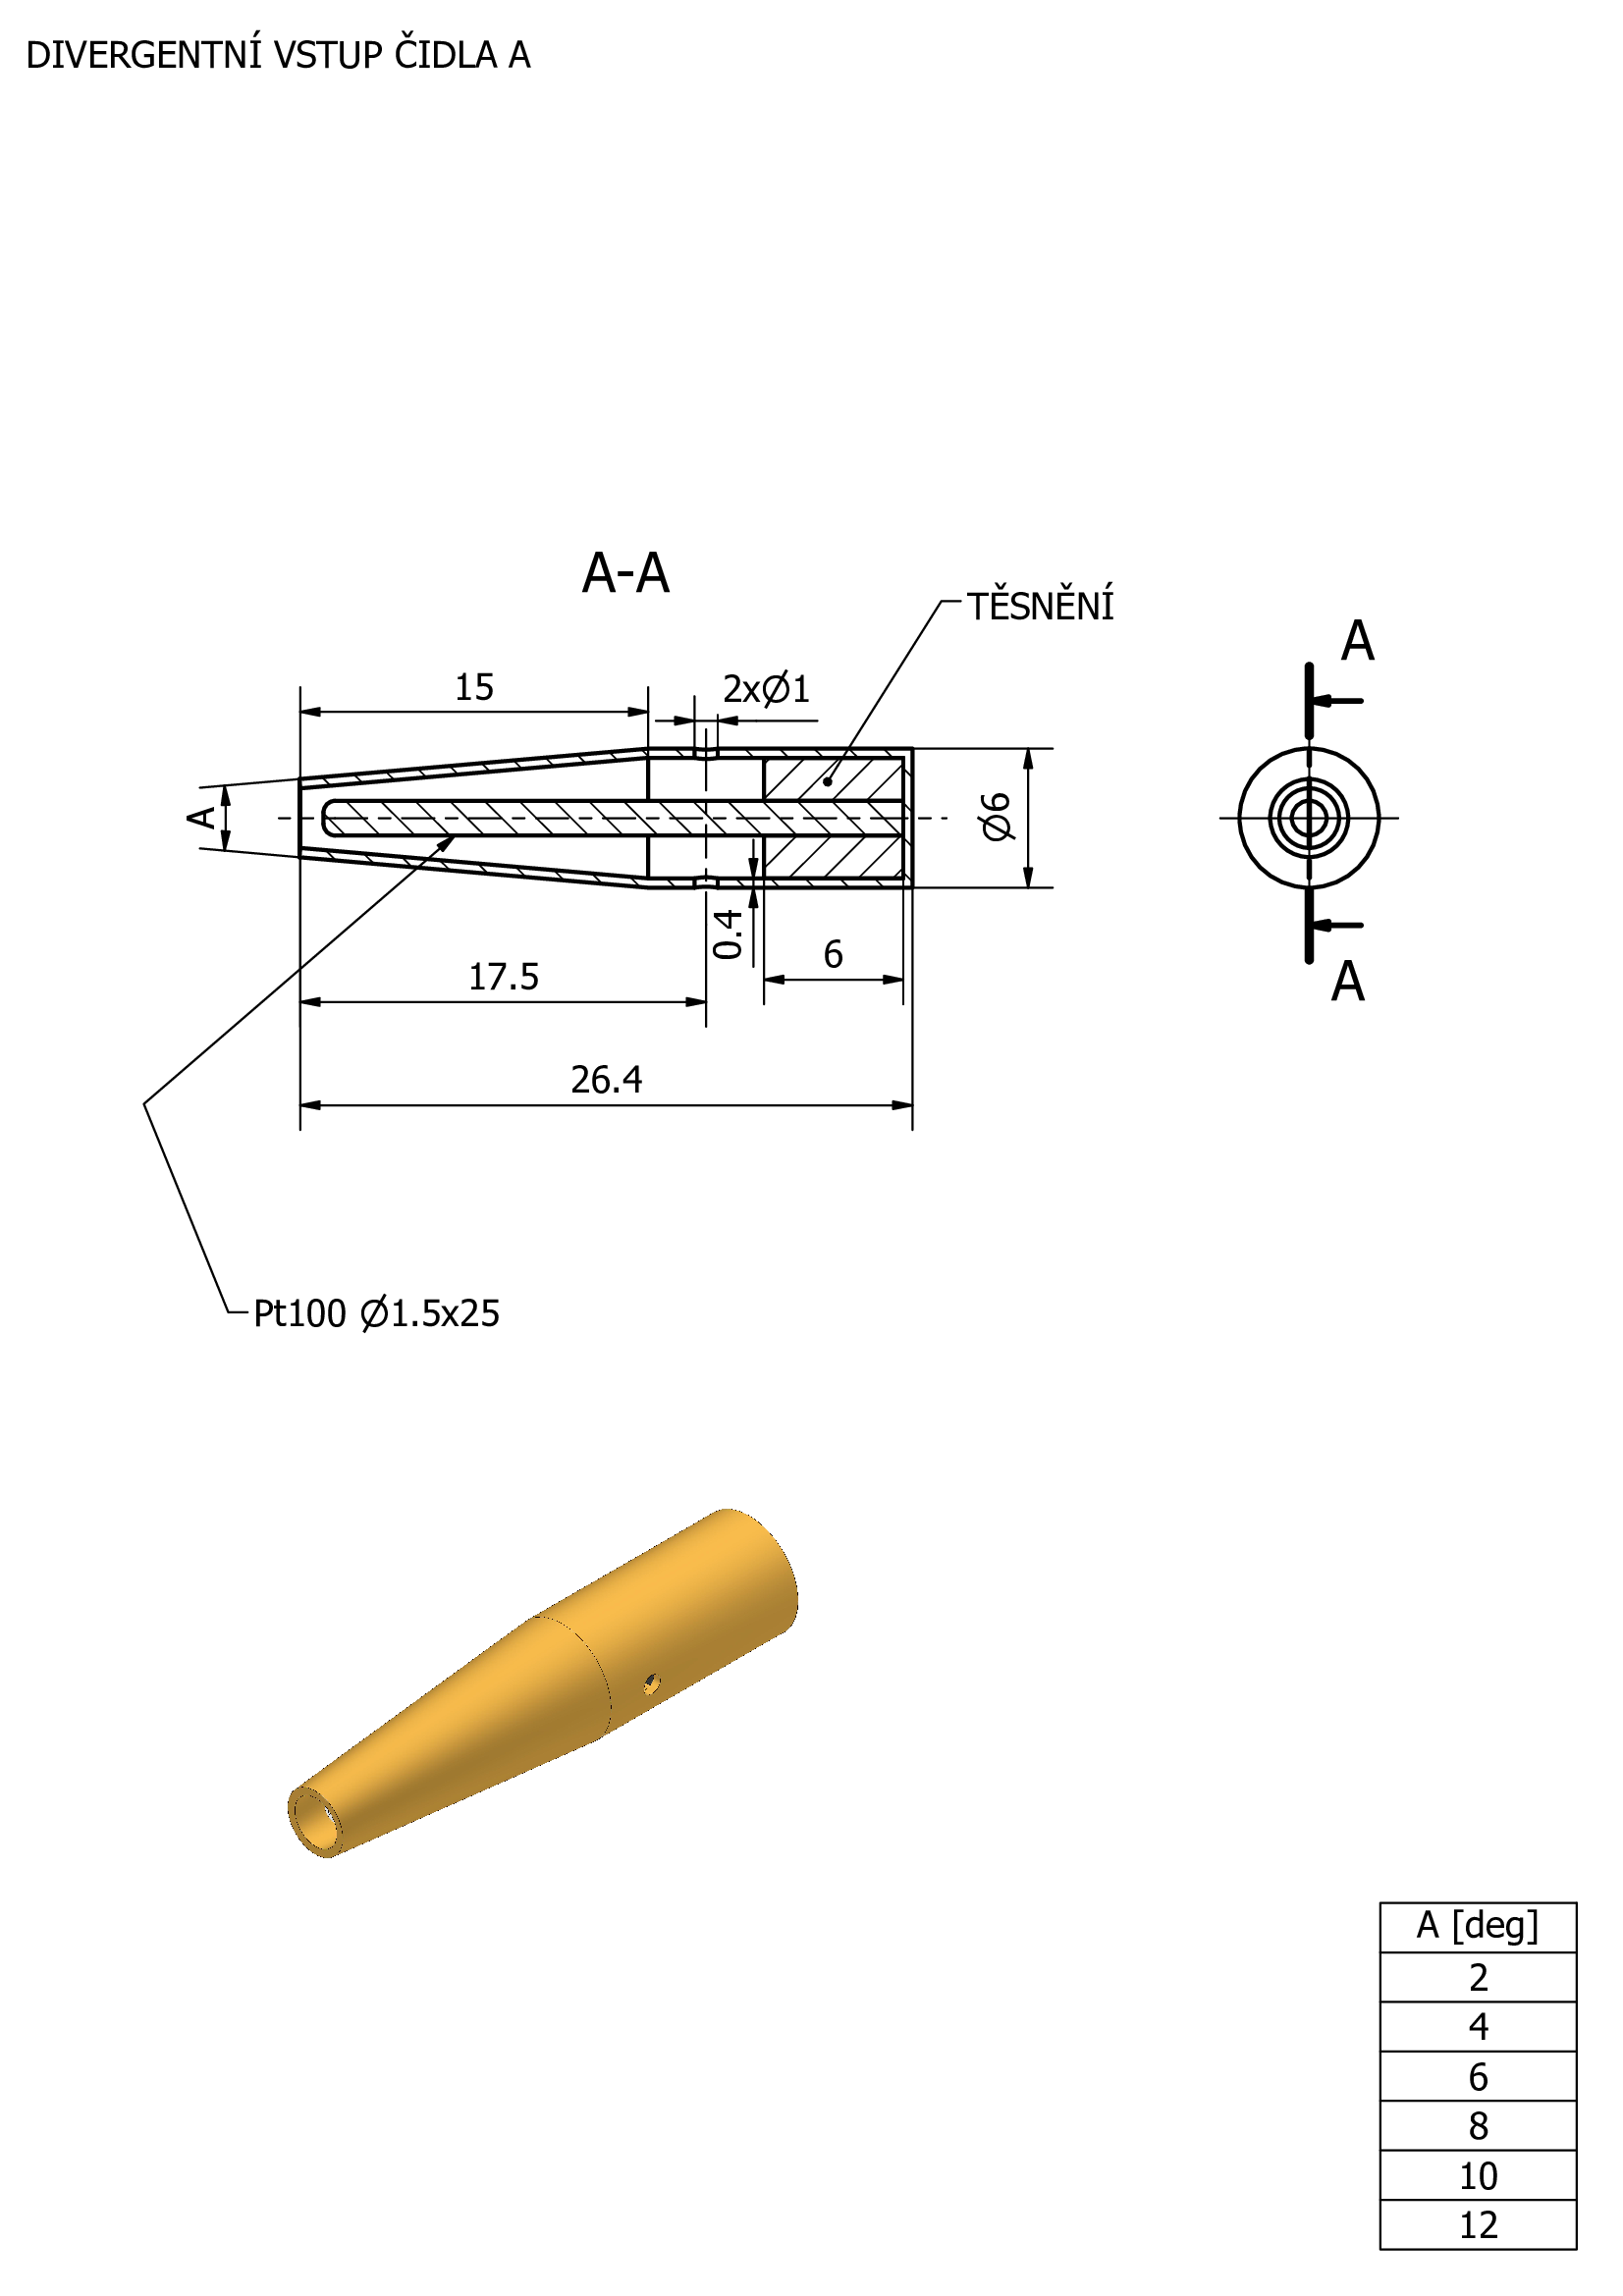
\includegraphics[width=\textwidth]{400_SIMULACE_KONSTRUKCNICH_UPRAV/Vykresy_rendery/Difuzor_A_vykres.png}
        
    \end{figure}
    \newpage
\sectionPriloha{Kavita ve stínění čidla A} \label{fig:kavita-A-vykres}
    \begin{figure}[ht!]
        \centering
        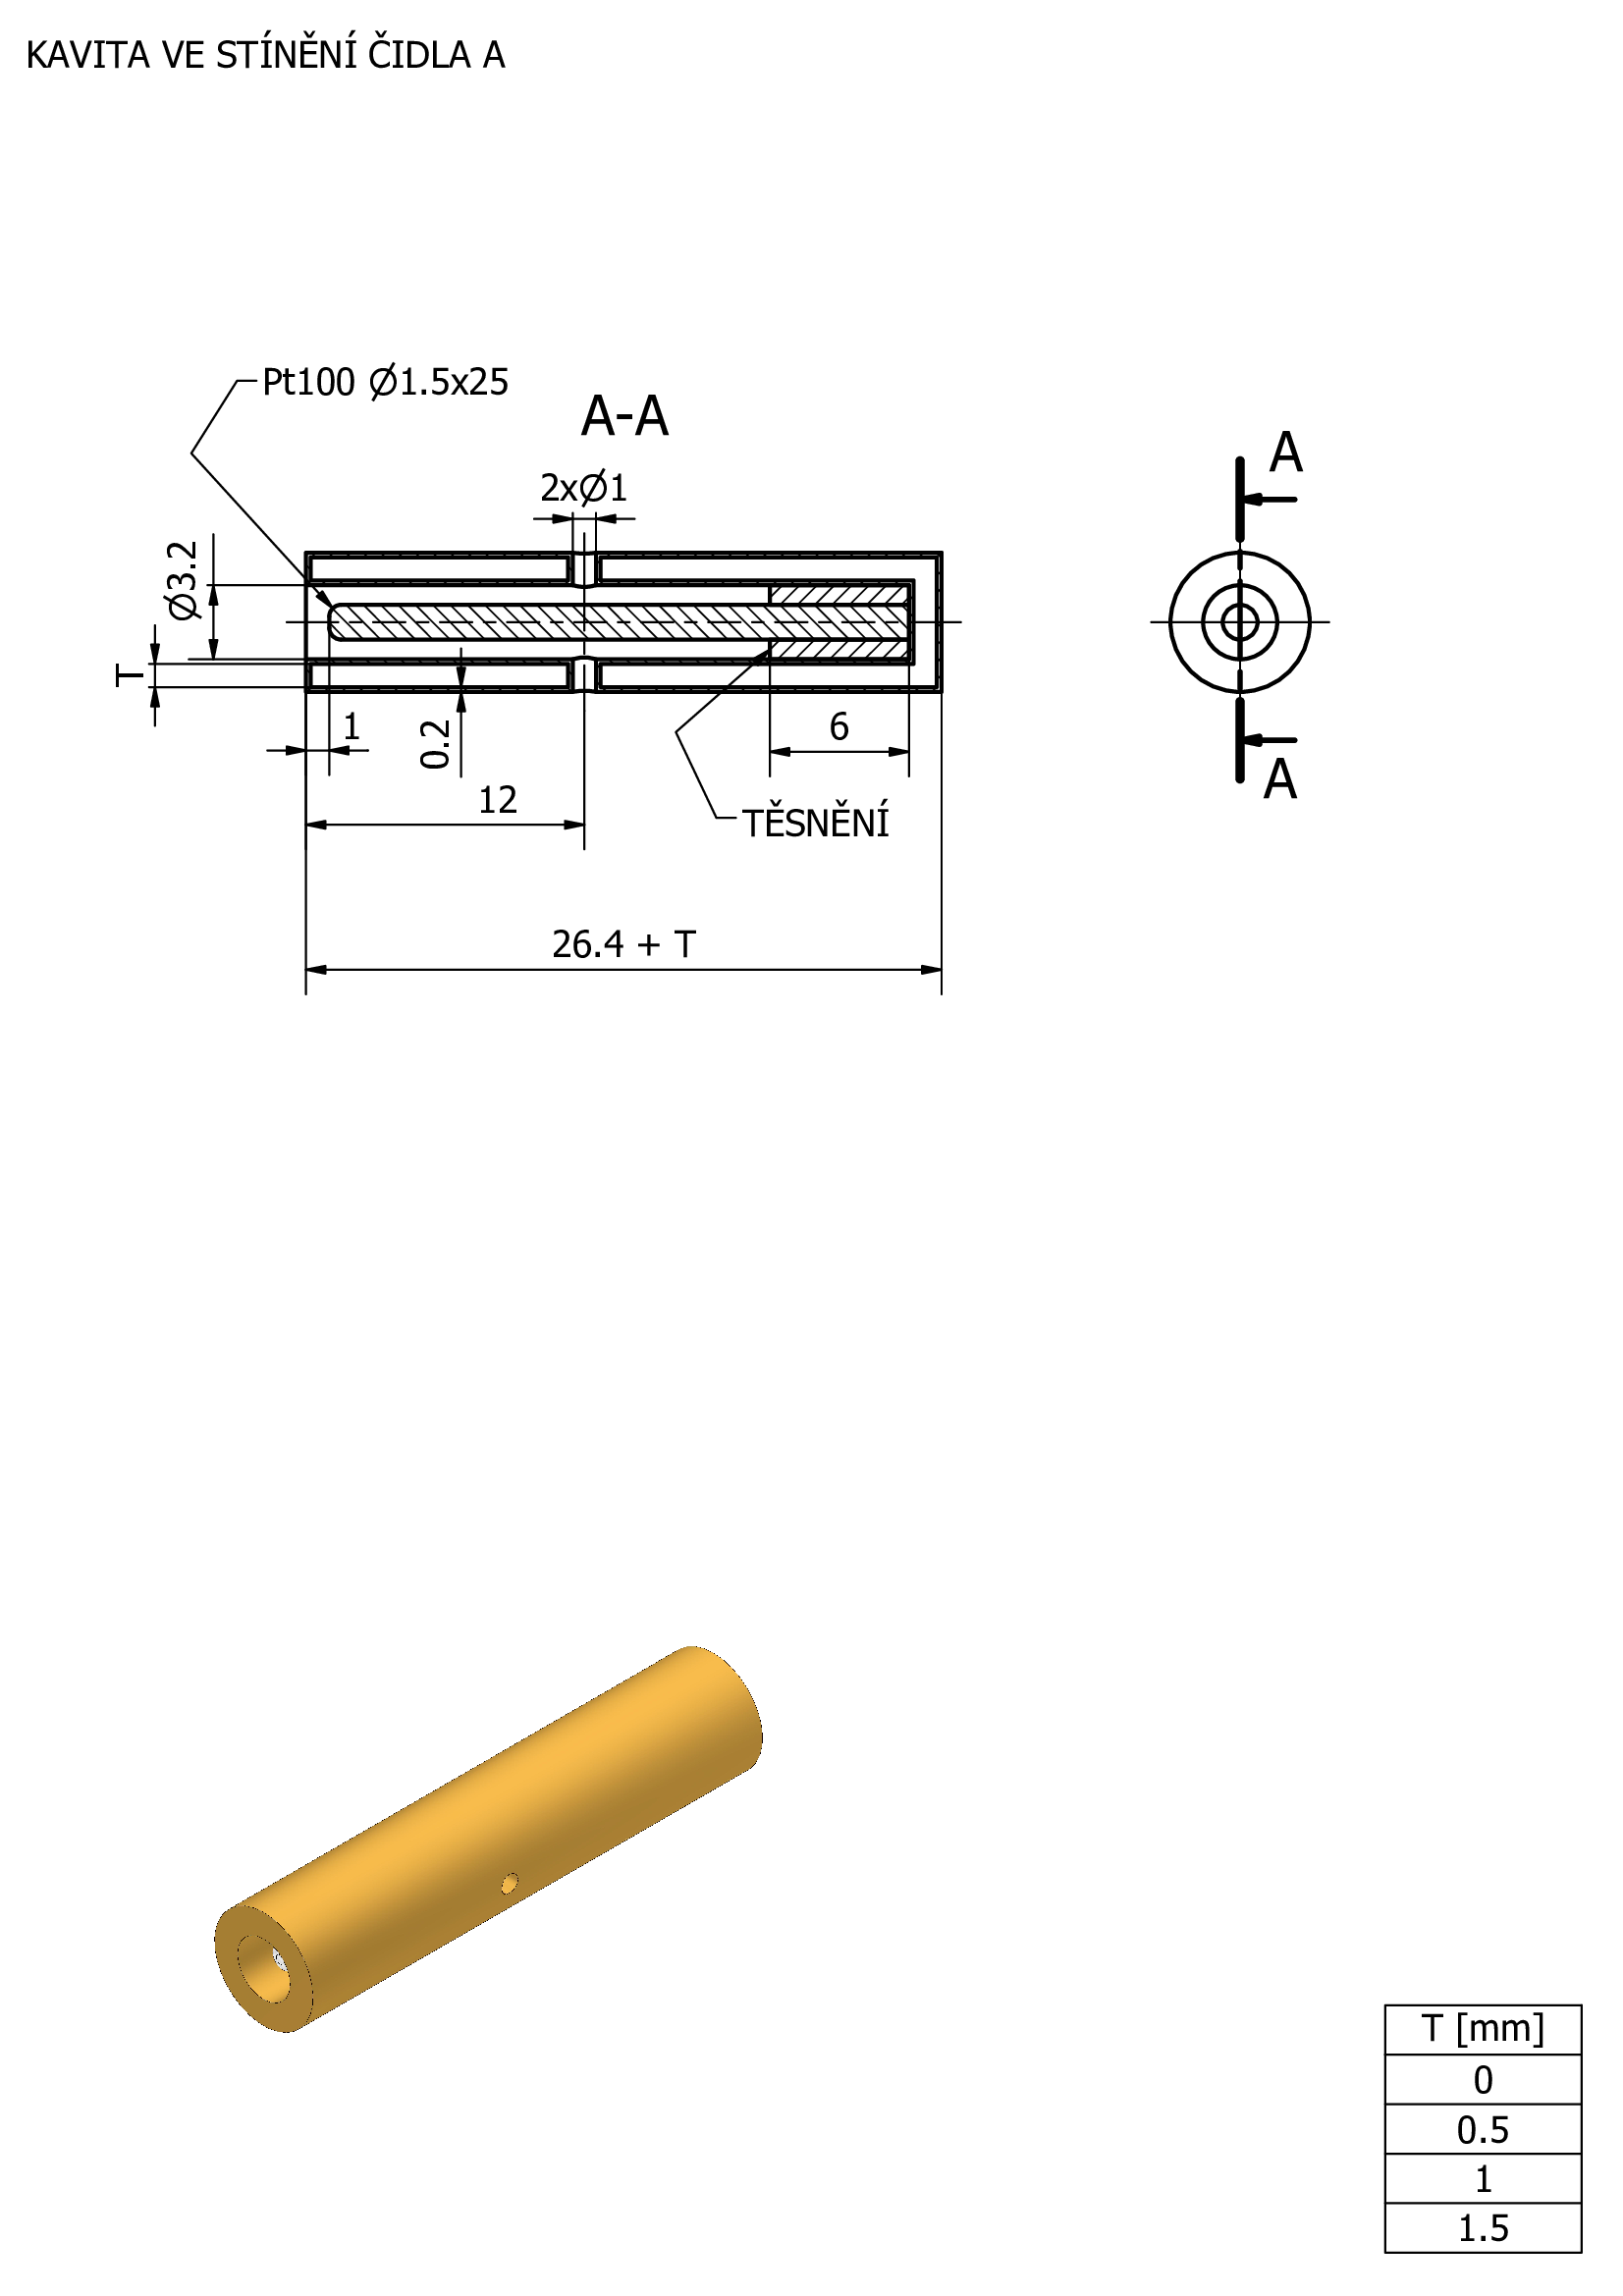
\includegraphics[width=\textwidth]{400_SIMULACE_KONSTRUKCNICH_UPRAV/Vykresy_rendery/Kavita_vykres.png}
    \end{figure}
    \newpage
\sectionPriloha{Kavita ve stínění čidla B} \label{fig:kavita-B-vykres}
    \begin{figure}[ht!]
        \centering
        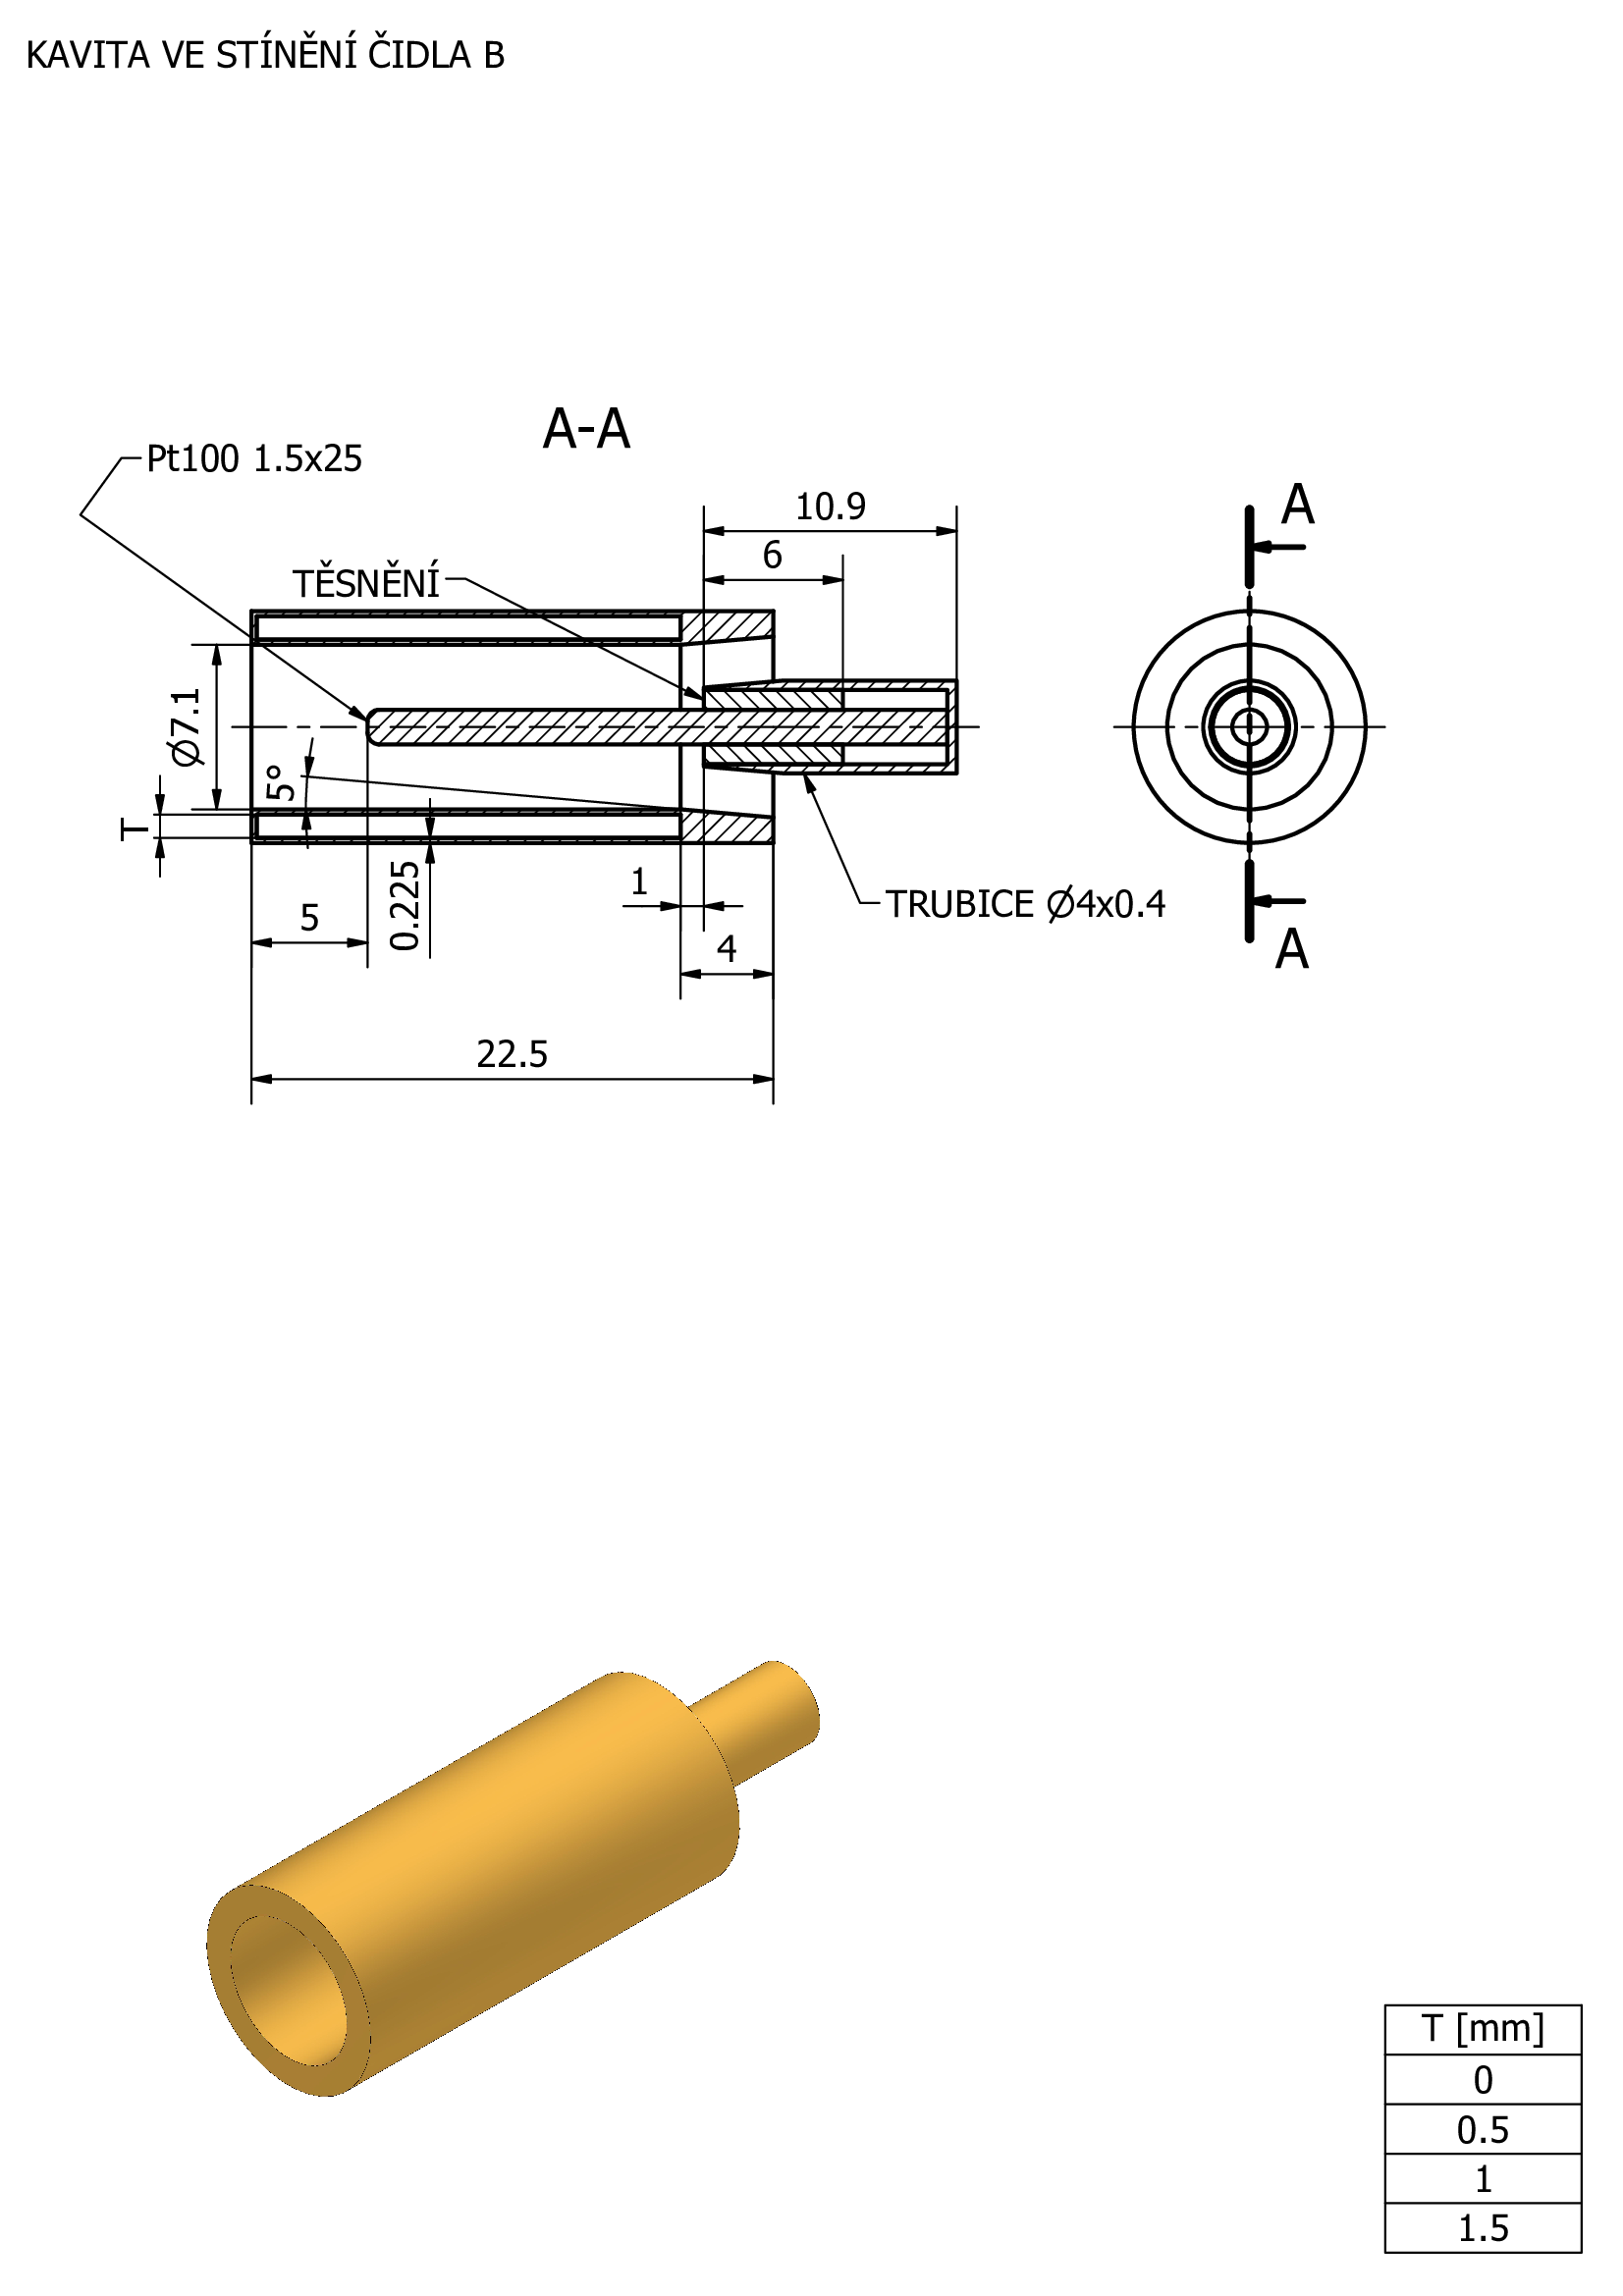
\includegraphics[width=\textwidth]{400_SIMULACE_KONSTRUKCNICH_UPRAV/Vykresy_rendery/Kavita_B_vykres.png}
    \end{figure}
\sectionPriloha{Finální verze sondy} \label{fig:sonda-final-vykres}
    \begin{figure}[ht!]
        \centering
        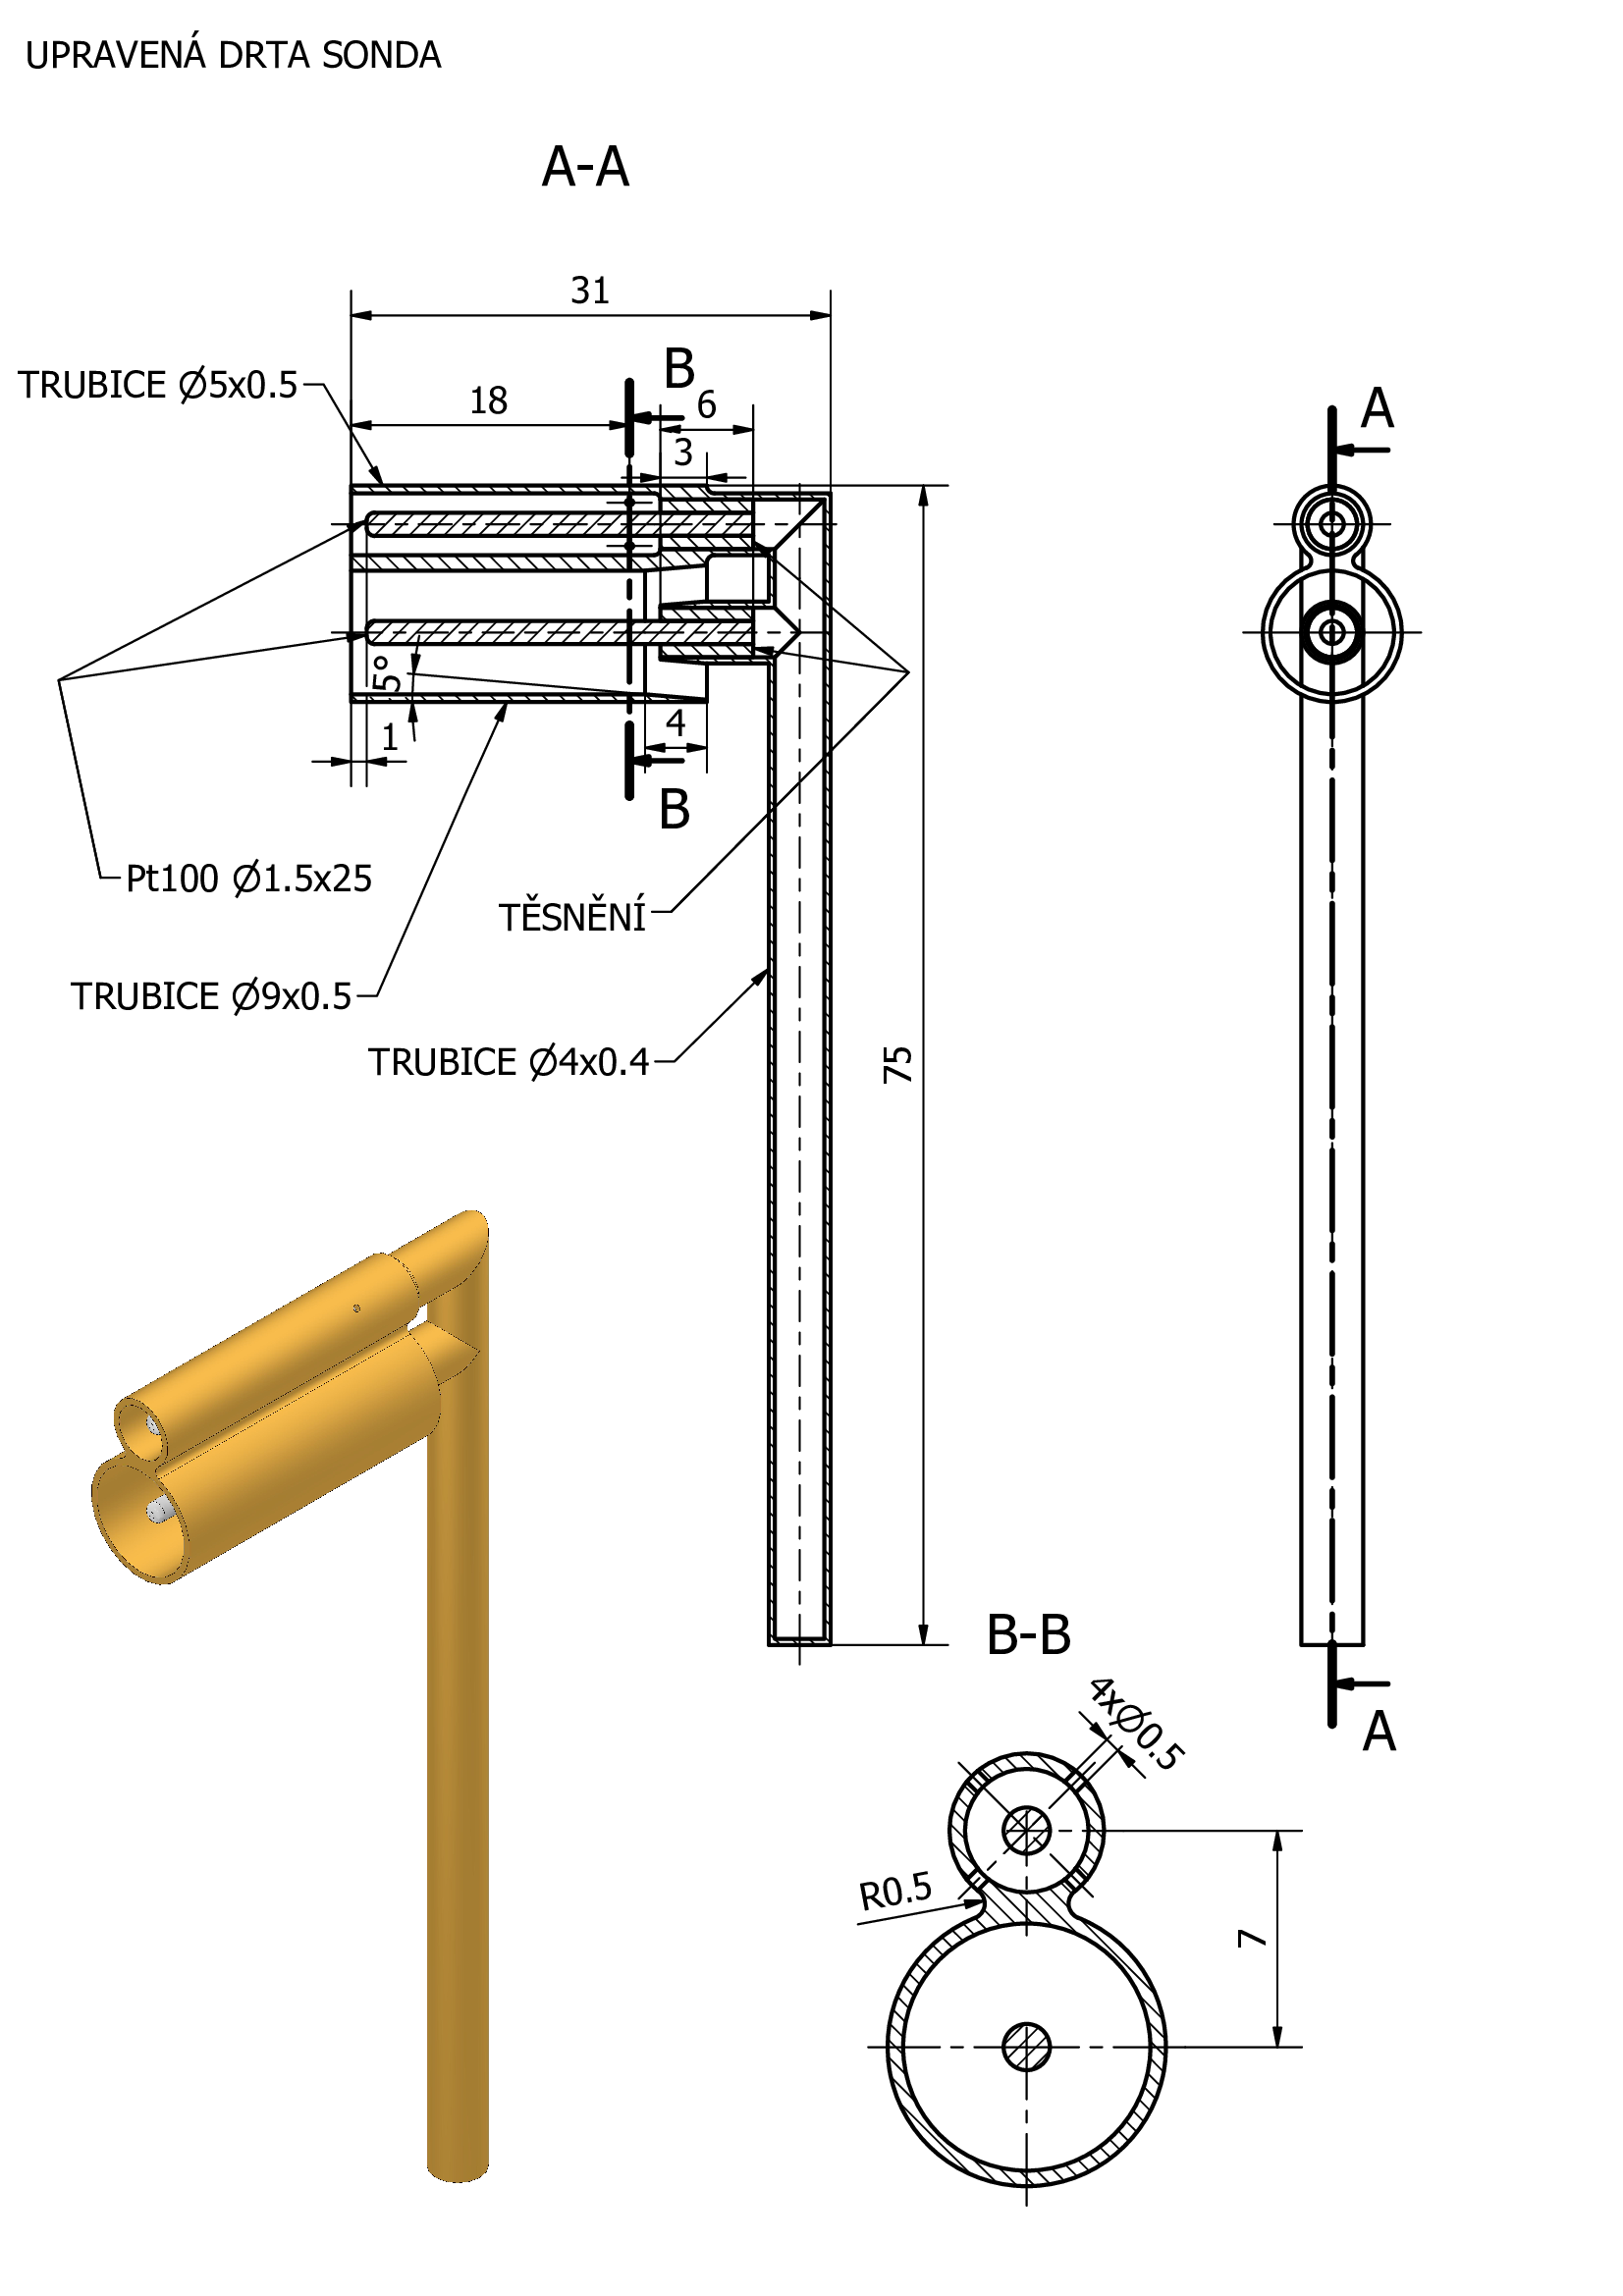
\includegraphics[width=\textwidth]{500_FINAL/sonda_final_vykres.png}
    \end{figure}

\sectionPriloha{Odvození chyby určení rychlosti při uvažování konstantního rozdílu restitučních faktorů} \label{sec:odvozeni-chyby}
    Pro účely odvození uvažujme následující veličiny:
    \begin{itemize}
        \item[–] $\Delta f$ skutečný rozdíl restitučních faktorů
        \item[–] $\Delta f_n$ jmenovitý rozdíl restitučních faktorů
        \item[–] $\delta f = \Delta f_n - \Delta f$ odchylku jmenovité a skutečné hodnoty rozdílu restitučních faktorů
        \item[–] $\Delta T_f$ rozdíl měřených teplot
        \item[–] $\overline{u} = \sqrt{\frac{2 c_p \Delta T_f}{\Delta f_n}}$ odhad rychlosti pomocí $\Delta f_n$
        \item[–] $u = \sqrt{\frac{2 c_p \Delta T_f}{\Delta f}}$ skutečnou rychlost
        \item[–] $\varepsilon _u = \frac{u - \overline{u}}{u}$ relativní chybu měření rychlosti
        \item[–] $\varepsilon _f = \frac{\delta f}{\Delta f}$ relativní odchylku skutečného a jmenovitého rozdílu restitučních faktorů
    \end{itemize}

    Vyjádřeme podíl odhadované a skutečné rychlosti jako funkce $\varepsilon _f$:
    \begin{equation*}
        \frac{\overline{u}}{u} = \frac{\sqrt{\frac{2 c_p \Delta T_f}{\Delta f_n}}}{\sqrt{\frac{2 c_p \Delta T_f}{\Delta f}}} = \sqrt{\frac{\Delta f}{\Delta  f + \delta f}} = \sqrt{\frac{1}{1 + \frac{\delta f}{\Delta f}}} = \sqrt{\frac{1}{1+\varepsilon _f}}
    \end{equation*}

    Nyní lze již jednoduše vyjádřit závislost $\varepsilon _u = \varepsilon _u \brac{\varepsilon _f}$:

    \begin{equation*}
        \varepsilon _u = \frac{u - \overline{u}}{u} = 1 - \frac{\overline{u}}{u} = 1 - \sqrt{\frac{1}{1+\varepsilon _f}}
    \end{equation*}